% Ce fichier main.tex est le fichier principal \`{a} partir duquel tout est g\'{e}n\'{e}r\'{e}
% This file is the main file where the final document is generated
\documentclass{these-dbl}

% Remplir les metadonnees du pdf
% Fill the pdf metadata
\hypersetup{
%    pdfauthor   = {XYZ},
%    pdftitle    = {Th\`{e}se de doctorat de XYZ},
%    pdfsubject  = {Th\`{e}se de doctorat de XYZ},
%    pdfkeywords = {mots-cl\'{e}s},
}

\geometry{vmargin=4.0cm}

% Spécifier vos fichiers de bibliographie
% Specify you bibliography files here
\addbibresource{./biblio.bib}

\providecommand{\tightlist}{%
  \setlength{\itemsep}{0pt}\setlength{\parskip}{0pt}}

\begin{document}
\pagenumbering{gobble}
% Page de garde avec commande \maketitle
% Front cover calling \maketitle
% La page de garde est en français
% The front cover is in French
\selectlanguage{french}
\pagenumbering{gobble}

% Inclure les infos de chaque établissement
% Include each institution data

%%% Switch case in latex
%%% https://tex.stackexchange.com/a/343306
\makeatletter
\newcommand\addcase[3]{\expandafter\def\csname\string#1@case@#2\endcsname{#3}}
\newcommand\makeswitch[2][]{%
    \newcommand#2[1]{%
        \ifcsname\string#2@case@##1\endcsname\csname\string#2@case@##1\endcsname\else#1\fi%
  }%
}
\makeatother

%%%% Il faut adapter la taille des logos dans certains cas (e.g., EGAAL, 2 etablissements)
\newcommand\hauteurlogos[3]{
    \hauteurlogoecole{#1}
    \hauteurlogoetablissementA{#2}
    \hauteurlogoetablissementB{#3}
}





%%%%%%%%%%%%%%%%%%%%%%%%%%%%%%%%%%%%%%%%%%%%%%%%%%%
%%%%%%%%%%%%%%%% ECOLES DOCTORALES %%%%%%%%%%%%%%%%

%%%% #1: dossier des images, #2: numero ED, #3: couleur ED recto, #4: couleur ED verso, #5-#6: nom complet sur plusieurs lignes
\newcommand\addecoledoctorale[6]{
    \direcole{#1}
    \numeroecole{#2}
    \definecolor{couleur-ecole-recto}{RGB}{#3}
    \definecolor{couleur-ecole-verso}{RGB}{#4}
    \nomecoleA{#5}
    \nomecoleB{#6}
}

\makeswitch[default]\ecoledoctorale{}

\addcase\ecoledoctorale{ALL}{\addecoledoctorale
    {ALL}
    {595}
    {255,165,139}
    {232,86,18}
    {Arts, Lettres, Langues}
    {}
}
\addcase\ecoledoctorale{DSP}{\addecoledoctorale
    {DSP}
    {599}
    {255,241,170}
    {255,214,12}
    {Droit et Science politiques}
    {}
}
\addcase\ecoledoctorale{EDGE}{\addecoledoctorale
    {EDGE}
    {597}
    {255,254,101}
    {255,237,0}
    {Sciences \'{e}conomiques et sciences de gestion - Bretagne}
    {}
}
\addcase\ecoledoctorale{EGAAL}{\addecoledoctorale
    {EGAAL}
    {600}
    {0,118,0}
    {0,93,49}
    {\'{E}cologie, G\'{e}osciences, Agronomie, Alimentation}
    {}
    \couleurpolice{white}
}
\addcase\ecoledoctorale{ELICCE}{\addecoledoctorale
    {ELICCE}
    {646}
    {255,207,114}
    {252,199,82}
    {\'{E}ducation, Langages, Interactions, Cognition, Clinique, Expertise}
    {}
}
\addcase\ecoledoctorale{ESC}{\addecoledoctorale
    {ESC}
    {645}
    {255,164,85}
    {240,138,0}
    {Espaces, Soci\'{e}\'{e}s, Civilisations}
    {}
}
\addcase\ecoledoctorale{MathSTICBO}{\addecoledoctorale
    {MathSTICBO}
    {644}
    {190,212,233}
    {139,181,221}
    {Math\'{e}matiques et Sciences et Technologies}
    {de l'Information et de la Communication en Bretagne Oc\'{e}ane}
}
\addcase\ecoledoctorale{MATISSE}{\addecoledoctorale
    {MATISSE}
    {601}
    {0,112,237}
    {0,84,160}
    {Math\'{e}matiques, T\'{e}l\'{e}communications, Informatique, Signal, Syst\`{e}mes,}
    {\'{E}lectronique}
    \hauteurlogos{1.8cm}{1.8cm}{1.8cm}
    \couleurpolice{white}
}
\addcase\ecoledoctorale{S3M}{\addecoledoctorale
    {S3M}
    {638}
    {159,19,90}
    {156,42,100}
    {Sciences de la Mati\`{e}re, des Mol\'{e}cules et Mat\'{e}riaux}
    {}
    \couleurpolice{white}
}
\addcase\ecoledoctorale{SML}{\addecoledoctorale
    {SML}
    {598}
    {19,139,112}
    {0,93,102}
    {Sciences de la Mer et du Littoral}
    {}
    \couleurpolice{white}
}
\addcase\ecoledoctorale{SPI}{\addecoledoctorale
    {SPI}
    {647}
    {136,191,255}
    {63,133,193}
    {Sciences pour l'Ing\'{e}nieur}
    {}
}
\addcase\ecoledoctorale{SPIN}{\addecoledoctorale
    {SPIN}
    {648}
    {161,173,255}
    {80,92,162}
    {Sciences pour l'Ing\'{e}nieur et le Num\'{e}rique}
    {}
}
\addcase\ecoledoctorale{SVS}{\addecoledoctorale
    {SVS}
    {637}
    {228,255,122}
    {200,210,0}
    {Sciences de la Vie et de la Sant\'{e}}
    {}
}





%%%%%%%%%%%%%%%%%%%%%%%%%%%%%%%%%%%%%%%%%%%%%%%%
%%%%%%%%%%%%%%%% ETABLISSEMENTS %%%%%%%%%%%%%%%%

%%%% #1 nom du logo, #2-#4: nom complet sur plusieurs lignes
\newcommand\addetablissement[4]{
    \logoetablissementB{#1}
    \nometablissementC{#2}
    \nometablissementD{#3}
    \nometablissementE{#4}
}

\makeswitch[default]\etablissement{}

\addcase\etablissement{CS}{\addetablissement
    {CS}
    {}
    {}
    {CentraleSup\'{e}lec}
}
\addcase\etablissement{EHESP}{\addetablissement
    {EHESP}
    {}
    {l'\'{E}cole des Hautes \'{E}tudes}
    {en Sant\'{e} Publique}
    \hauteurlogos{2cm}{}{2.5cm}
}
\addcase\etablissement{ENIB}{\addetablissement
    {ENIB}
    {}
    {}
    {l'\'{E}cole Nationale d'Ing\'{e}nieurs de Brest}
}
\addcase\etablissement{ENS}{\addetablissement
    {ENS}
    {}
    {}
    {l'\'{E}cole Normale Sup\'{e}rieure de Rennes}
}
\addcase\etablissement{ENSAI}{\addetablissement
    {ENSAI}
    {}
    {l'\'{E}cole Nationale de la Statistique}
    {et de l'Analyse de l'Information}
}
\addcase\etablissement{ENSCR}{\addetablissement
    {ENSCR}
    {}
    {l'\'{E}cole Nationale Sup\'{e}rieure}
    {de Chimie Rennes}
}
\addcase\etablissement{ENSTA}{\addetablissement
    {ENSTA}
    {}
    {l'\'{E}cole Nationale Sup\'{e}rieure}
    {de Techniques Avanc\'{e}es Bretagne}
}
\addcase\etablissement{IMTA}{\addetablissement
    {IMTA}
    {l'\'{E}cole Nationale Sup\'{e}rieure}
    {Mines-T\'{e}l\'{e}com Atlantique Bretagne}
    {Pays de la Loire -- IMT Atlantique}
}
\addcase\etablissement{INSA}{\addetablissement
    {INSA}
    {}
    {l'Institut National des}
    {Sciences Appliqu\'{e}es de Rennes}
    \hauteurlogos{1.8cm}{}{2cm}
}
\addcase\etablissement{InstitutAgro}{\addetablissement
    {InstitutAgro}
    {}
    {}
    {l'Institut Agro Rennes Angers}
}
\addcase\etablissement{UBO}{\addetablissement
    {UBO}
    {}
    {}
    {l'Universit\'{e} de Bretagne Occidentale}
}
\addcase\etablissement{UBS}{\addetablissement
    {UBS}
    {}
    {}
    {l'Universit\'{e} Bretagne Sud}
}
\addcase\etablissement{UR}{\addetablissement
    {UR}
    {}
    {}
    {l'Universit\'{e} de Rennes}
}
\addcase\etablissement{UR2}{\addetablissement
    {UR2}
    {}
    {}
    {l'Universit\'{e} Rennes 2}
}

%%%% #1-#2: nom des deux logos, #3-#7: nom complet de la double affiliation sur plusieurs lignes
\newcommand\addpairetablissements[7]{
    \logoetablissementA{#1}
    \logoetablissementB{#2}
    \nometablissementA{#3}
    \nometablissementB{#4}
    \nometablissementC{#5}
    \nometablissementD{#6}
    \nometablissementE{#7}
}

% ALL, ESC: ENSAB-UR2
\addcase\etablissement{ENSAB-UR2}{\addpairetablissements
    {ENSAB}
    {UR2}
    {}
    {l'\'{E}cole Nationale Sup\'{e}rieure}
    {d'Architecture de Bretagne}
    {d\'{e}livr\'{e}e conjointement avec}
    {l'Universit\'{e} Rennes 2}
    \hauteurlogos{2cm}{1.2cm}{2cm}
}
% DSP, MATISSE, SVS: UR2-UR
\addcase\etablissement{UR2-UR}{\addpairetablissements
    {UR2}
    {UR}
    {}
    {}
    {l'Universit\'{e} Rennes 2}
    {d\'{e}livr\'{e}e conjointement avec}
    {l'Universit\'{e} de Rennes}
    \hauteurlogos{1.8cm}{1.8cm}{1.5cm}
}
% DSP, EDGE: EHESP-UR
\addcase\etablissement{EHESP-UR}{\addpairetablissements
    {EHESP}
    {UR}
    {}
    {l'\'{E}cole des Hautes \'{E}tudes}
    {en Sant\'{e} Publique}
    {d\'{e}livr\'{e}e conjointement avec}
    {l'Universit\'{e} de Rennes}
    \hauteurlogos{2cm}{2cm}{1.5cm}
}
% MATISSE: InstitutAgro-UR
\addcase\etablissement{InstitutAgro-UR}{\addpairetablissements
    {InstitutAgro}
    {UR}
    {}
    {l'Institut Agro}
    {Rennes Angers}
    {d\'{e}livr\'{e}e conjointement avec}
    {l'Universit\'{e} de Rennes}
    \hauteurlogos{1.8cm}{1.2cm}{1.2cm}
}
% SPI: ENIB-UBO
\addcase\etablissement{ENIB-UBO}{\addpairetablissements
    {ENIB}
    {UBO}
    {}
    {l'\'{E}cole Nationale}
    {d'Ing\'{e}nieurs de Brest}
    {d\'{e}livr\'{e}e conjointement avec}
    {l'Universit\'{e} de Bretagne Occidentale}
    \hauteurlogos{2cm}{1.6cm}{1.6cm}
}


% Inclure infos de l'école doctorale
% Include doctoral school data
\ecoledoctorale{SML}

% Inclure infos de l'établissement
% Include institution data
\etablissement{UBO}

%Inscrivez ici votre sp\'{e}cialit\'{e} (voir liste des sp\'{e}cialit\'{e}s sur le site de votre \'{e}cole doctorale)
%Indicate the domain (see list of domains in your ecole doctorale)
\spec{Ecologie Marine}

%Attention : le pr\'{e}nom doit être en minuscules (Jean) et le NOM en majuscules (BRITTEF) 
%Attention : the first name in small letters and the name in Capital letters 
\author{Clément VIOLET}

% Donner le titre complet de la th\`{e}se, \'{e}ventuellement le sous titre, si n\'{e}cessaire sur plusieurs lignes 
%Give the complete title of the thesis, if necessary on several lines
\title{« Titre de la th\`{e}se »}
\lesoustitre{« Sous-titre de la th\`{e}se »}

%Indiquer la date et le lieu de soutenance de la th\`{e}se 
%indicates the date and the place of the defense 
\date{« date »}
\lieu{« Lieu »}

%Indiquer le nom du (ou des) laboratoire (s) dans le(s)quel(s) le travail de th\`{e}se a \'{e}t\'{e} effectu\'{e}, indiquer aussi si souhait\'{e} le nom de la (les) facult\'{e}(s) (UFR, \'{e}cole(s), Institut(s), Centre(s)...), son (leurs) adresse(s)... 
%Indicates the name (or names) of research laboratories where the work has been done as well as (if desired) the names of faculties (UFR, Schools, institution...
\uniterecherche{Ifremer - DYNECO-LEBCO}

%Indiquer le Numero de th\`{e}se, si cela est opportun, ou laisser vide pour faire disparaitre cet ligne de la couverture
%Indicate the number of the thesis if there is one. otherwise leave empty so the line disappeurs on the cover
\numthese{« si pertinent »} % \numthese{}

%Indiquer le Pr\'{e}nom en minuscules et le Nom en majuscules, le titre de la personne et l’\'{e}tablissement dans lequel il effectue sa recherche  
%Indicates the first name on small letters and the Names on capital letters, the person's title and the institution where he/she belongs to.
%Exemples :  Examples :
%%%- Professeur, Universit\'{e} d’Angers 
%%%- Chercheur, CNRS, \'{e}cole Centrale de Nantes 
%%%-  Professeur d’universit\'{e} – Praticien Hospitalier, Universit\'{e} Paris V  
%%%-  Maitre de conf\'{e}rences, Oniris 
%%%- Charg\'{e} de recherche, INSERM, HDR, Universit\'{e} de Tours  
 %S’il n’y a pas de co-direction, faire disparaitre cet item de la couverture  
 %In there is no co-director, remove the item from the cover
\jury{
{\normalTwelve \textbf{Rapporteurs avant soutenance :}}\\ \newline
\footnotesizeTwelve
\begin{tabular}{@{}ll}
Pr\'{e}nom NOM & Fonction et \'{e}tablissement d'exercice \\
Pr\'{e}nom NOM & Fonction et \'{e}tablissement d'exercice \\
Pr\'{e}nom NOM & Fonction et \'{e}tablissement d'exercice \\
\end{tabular}

\vspace{\baselineskip}
{\normalTwelve \textbf{Composition du Jury :}}\\
{\fontsize{9.5}{11}\selectfont {\textcolor{red}{\textit{Attention, en cas d’absence d’un des membres du Jury le jour de la soutenance, la composition du jury doit être revue pour s’assurer qu’elle est conforme et devra être répercutée sur la couverture de thèse}}}}\\ \newline
\footnotesizeTwelve
\begin{tabular}{@{}lll}

Pr\'{e}sident :        & Pr\'{e}nom NOM & Fonction et \'{e}tablissement d'exercice \textit{(à préciser après la soutenance)} \\
Examinateurs :         & Pr\'{e}nom NOM & Fonction et \'{e}tablissement d'exercice \\
                       & Pr\'{e}nom NOM & Fonction et \'{e}tablissement d'exercice \\
                       & Pr\'{e}nom NOM & Fonction et \'{e}tablissement d'exercice \\
                       & Pr\'{e}nom NOM & Fonction et \'{e}tablissement d'exercice \\
Dir. de th\`{e}se :    & Pr\'{e}nom NOM & Fonction et \'{e}tablissement d'exercice \\
Co-dir. de th\`{e}se : & Pr\'{e}nom NOM & Fonction et \'{e}tablissement d'exercice \textit{(si pertinent)} \\
\end{tabular}

\vspace{\baselineskip}
{\normalTwelve \textbf{Invit\'{e}(s) :}}\\ \newline
\footnotesizeTwelve
\begin{tabular}{@{}ll}
Pr\'{e}nom NOM & Fonction et \'{e}tablissement d'exercice \\
\end{tabular}
}


\maketitle


% Sélectionner la langue du contenu suivant cette ligne
% Select the content language following this line
\selectlanguage{french}

% Inclusion du chapitre remerciement
% Input acknowledgement chapter
\clearemptydoublepage
\hypertarget{remerciements}{%
\chapter*{Remerciements}\label{remerciements}}

Je tiens à remercier I would like to thank. my parents.. J'adresse
également toute ma reconnaissance à \ldots. \ldots.


\clearemptydoublepage
% Ne pas oublier cette commande qui g\'{e}n\`{e}re la page de couverture avant
% This command will generate the front cover
\frontmatter
% \renewcommand{\contentsname}{Table of Contents}
\tableofcontents %sommaire %table of content
\listoffigures
\listoftables
%\shorttableofcontents{Sommaire}{0}

\clearemptydoublepage
\pagenumbering{arabic}
\hypertarget{introduction}{%
\chapter*{Introduction}\label{introduction}}
\addcontentsline{toc}{chapter}{Introduction}

\chaptermark{Introduction}

\hypertarget{les-uxe9costysuxe8mes-cuxf4tiers}{%
\section*{Les écostysèmes
côtiers}\label{les-uxe9costysuxe8mes-cuxf4tiers}}
\addcontentsline{toc}{section}{Les écostysèmes côtiers}

La notion d'habitat est essentielle en écologie. Cette notion englobe
non seulement le lieu où une espèce peut être trouvée, le(s) lieu(x) où
elle réalise son cycle de vie, mais également l'ensemble des conditions
abiotiques et biotiques qui permettent le maintien de sa population
\autocite{Hall_1997}. Certaines espèces animales ou végétales ont la
capacité de modifier leur environnement de nombreuses façons
différentes, comme en modifiant les conditions environnementales
\autocite{Ellison_2019} ou en produisant des structures
tridimensionnelles complexes permettant d'abriter d'autres espèces
\autocite{Darling_2017}. Ces espèces sont qualifiées d'espèces
ingénieurs \autocite{Jones_1996}. Ces espèces ingénieurs peuvent de par
leur seule présence caractériser un habitat, c'est pourquoi dans la
suite de ce manuscrit, nous allons qualifier les habitats créés par ces
espèces d'habitats biogéniques.

Les habitats biogéniques structurent la dynamique des écosystèmes
benthiques côtiers auxquels elles sont associées \autocites[
]{Duffy_2006}{Teagle_2017}. Ces habitats vont promouvoir une plus grande
diversité spécifique au sein des écosystèmes qui les abritent
\autocites[ ]{Romero_2015}{Sunday_2016}, notamment de par leur capacité
à tamponner les conditions environnementales locales en modifiant par
exemple la température \autocite{Bulleri_2018}. A une échelle locale,
les habitats biogéniques tendent donc à augmenter l'hétérogénéité
spatiale de l'environnement et par conséquent augmentent la diversité et
l'abondance de niches environnementales disponibles pour d'autres
espèces \autocites[ ]{Duffy_2006}{Hewitt_2005}. Ces modifications
locales de l'environnement par les habitats biogéniques entretiennent
des boucles de rétroactions négatives \autocite{Kefi_2016}, ces boucles
de rétroactions négatives ont des effets stabilisateurs des conditions
environnementales, ce qui à une échelle globale augmente la résilience
des écosystèmes face aux perturbations entraînées par le changement
climatique global (fig.~\ref{fig:1}; \textcite{Bulleri_2018} ;
\textcite{Jurgens_2022}). Un exemple simplifié est celui des herbiers
marins, qui assurent la protection des mezobrouteur\footnote{Les
  mezobrouteurs sont de petits invertébrés herbivores d'une taille
  inférieure ou égale à 2,5 cm \autocite{Beermann_2018}.} contre leurs
prédateurs, qui vont se nourrir des épiphytes permettant à l'herbier de
se maintenir et de s'agrandir. Ainsi, ces boucles de rétroactions
négatives ont des effets stabilisateurs des conditions
environnementales, ce qui à une échelle globale augmente la résilience
des écosystèmes face aux perturbations entraînées par le changement
climatique global \autocites[ ]{Bulleri_2018}{Jurgens_2022}.

La promotion de la biodiversité par les habitats biogéniques a également
un impact sur les services écosystémiques fournis par les écosystèmes
marins. Ces habitats biogéniques sont notamment des zones importantes
pour le cycle de vie de poissons à forte valeur commerciale. Par
exemple, les prés-salés et les herbiers marins sont des zones de
nourricerie essentielles au développement des juvéniles comme ceux du
bar commun (\emph{Dicentrarchus labrax}) \autocites[
]{Stamp_2022}{Maxwell_2017}. Ces habitats biogéniques ont également un
fort impact économique ; les récifs coralliens supportent par exemple
une industrie du tourisme conséquente (valeur estimée à près de
36~milliards de dollars par an ; \textcite{Spalding_2017}). Enfin, les
habitats biogéniques jouent un rôle particulièrement important dans la
lutte contre l'érosion, via leur effet de stabilisation du sédiment
\autocite{Reidenbach_2018} ou bien en réduisant l'énergie des vagues
lors d'évènements extrêmes comme les tempêtes \autocite{Krauss_2019} ou
bien les tsunamis \autocite{Alongi_2008}.

Malgré leur importance, les écosystèmes côtiers font face à de
nombreuses menaces comme l'acidification des océans
\autocite{Doney_2009}, l'augmentation des températures
\autocite{IPCC_2021_technical_summary}, l'augmentation du nombre et de
la fréquence des évènements climatiques extrêmes \autocite{Oliver_2018},
ainsi que de leur surexploitation \autocites[ ]{Lotze_2006}{Lotze_2009}.
Ainsi, les habitats biogéniques qui sont de nature souvent fragile, car
formés par des espèces souvent sensibles aux différents impacts
anthropiquesont et ont décliné tant en qualité (i.e.~dégradation de
l'état écologique, ou perte de complexité, etc.), qu'en quantité
(i.e.~souvent exprimé comme une réduction de leur superficie) à travers
l'Europe et dans le monde entier \autocites[ ]{Airoldi_2007}[
]{Dunic_2021}[ ]{McCauley_2015}{Waycott_2009}. Ces pertes des habitats
biogéniques sont l'un des principaux moteurs du déclin de la
biodiversité auquel nous assistons actuellement \autocites[
]{Airoldi_2007}[ ]{ipbes_2019}{McCauley_2015}.

Ces différentes pressions d'origine anthropique et leurs conséquences
sur les habitats biogéniques vont affecter par effet de cascade
fonctionnement et dynamique globale des écosystèmes côtiers \autocites[
]{Rocha_2015a}[ ]{Sara_2021}{Wernberg_2016}. Les écosystèmes étant des
objets dynamiques, ils peuvent répondre de différente manière à ces
pressions. Après avoir dépassé leur seuil de résistance envers ces
perturbations, ils vont être transformés de façon linéaire, ou bien de
manière non linéaire. Ces changements non linéaires entraînent des
modifications profondes des écosystèmes appelés ``changement de régime''
\autocite{Scheffer_2001}. Dans le cas des transitions linéaires, il
serait possible d'identifier des états d'habitats différents de l'état
pristin plus ou moins dégradé \autocite{Spake_2022}. Lorsque les
transformations suivent des tendances non linéaires, l'apparition de
seuils empêchera le retour à l'état pristin des écosystèmes
\autocite{Spake_2022}.

Ces changements de régimes et d'états ont d'ores et déjà été observés à
travers un grand nombre d'écosystèmes terrestres et marins, par exemple
: la transition entre la toundra et la forêt boréale
\autocite{Folke_2004}, entre la forêt et la savane \autocites[
]{Debra_2004}{Folke_2004}, mais également, comme pour les forêts de
laminaires qui peuvent laisser place à des déserts d'oursins \autocites[
]{Carnell_2020}{Rogers-Bennett_2019}, ou bien encore les récifs
coralliens supplantés par des macroalgues \autocites[
]{Folke_2004}{OBrien_2018}. Le déclin des habitats biogénique est
notamment l'un des moteurs des changements de régimes observés ces
dernières décennies \autocites[ ]{Rocha_2015a}{Wernberg_2016}.

Pour éviter la dégradation des écosystèmes marins liée à la disparition
des habitats biogéniques, les écologues font face à de nombreux défis à
relever. Un premier défi consiste à identifier et décrire les différents
types d'habitats biogéniques à l'échelle mondiale de façon adéquate pour
identifier les changements d'état d'habitat. En effet, les typologies
existantes ont du mal à détecter ces changements \autocite{Cooper_2019},
ce qui entrave la mise en place de mesures de gestion efficaces
\autocite{Ware_2020}. Par conséquent, il est essentiel de développer une
typologie d'habitat mondiale basée sur les suivis biologiques existants
\autocite{Cooper_2019} afin de mieux coordonner les politiques de
préservation des habitats côtiers \autocite{Ware_2020}. Le second défi
réside dans la prévention des changements d'état d'habitats biogéniques.
Pour ce faire, il est nécessaire d'identifier les facteurs externes et
internes qui contribuent d'une part à leur résilience et d'autre part
qui facilitent les transitions vers d'autres types d'habitats. Grâce à
une meilleure connaissance de ces facteurs, il sera possible
d'identifier des zones géographiques plus à risque de changement de
régime, et donc de mettre en place des mesures de suivi adéquat
permettant de réagir dès les premiers signes de changement de régime
observés.

Le développement de nouveaux outils méthodologiques de modélisation peut
permettre de faire face au premier défi. Pour le second, deux approches
différentes existent : une expérimentale, grâce à des expérimentations
\emph{in situ} ou en méscosome et une approche de modélisation. Ces
expérimentations \emph{in situ} ou en mésocosme présentent certains
avantages comme celui d'avoir une observation directe des phénomènes
étudiés \autocite{Fulton_2019}. Cependant, elles sont souvent réalisées
à des échelles spatiales restreintes et sur des périodes de temps
limitées, particulièrement lorsque les études s'intéressent aux
écosystèmes marins du fait de leurs contraintes \autocite{Witman_2015}.
Ainsi, les interactions entre les organismes, les conditions
environnementales et les pressions observées lors de ces
expérimentations peuvent être différentes de ce qui passe à plus large
échelle spatiale et/ou temporelle. Les résultats de ces expérimentations
peuvent alors être plus difficilement généralisables
\autocite{Witman_2015}.

Pour surmonter ces contraintes, l'utilisation d'outils de modélisation
peut se révéler utile. Les modèles sont des représentations simplifiées
des systèmes écologiques qui permettent leur étude à des échelles
spatiotemporelles plus grandes. Les modèles en écologie peuvent être
regroupés en deux catégories : de manière mécanistique ou corrélatives
\autocite{Kearney_2010}. Ces modèles peuvent être complexifiés à loisir
selon les hypothèses de recherche pour mieux prendre en compte la
complexité réelle des écosystèmes \autocite{Cartwright_2016}. Les
modèles permettent également de prédire les changements futurs des
habitats biogéniques en fonction des scénarios de changement climatique
\autocite{Curd_2023}.

L'objectif principal de cette thèse est d'améliorer la compréhension et
la prévision des changements potentiels dans les habitats biogéniques
des environnements benthiques côtiers. Pour cela, elle se concentre sur
l'identification des types d'habitats benthiques, l'exploration de leurs
états alternatifs et l'analyse des facteurs favorisant l'établissement
de ces différents états. Afin d'atteindre cet objectif, la thèse
s'appuie sur les données collectées par le programme \emph{Reef Life
Survey}, qui a effectué depuis 2008 des suivis des habitats et de la
faune des récifs côtiers à travers le monde. Grâce à ces données, la
thèse vise à identifier les principaux types d'habitats benthiques
côtiers en développant de nouvelles méthodes pouvant être adaptées à
d'autres écosystèmes. Elle contribue également à acquérir de nouvelles
connaissances sur les facteurs environnementaux et les pressions
d'origine humaine qui influent sur le maintien ou le changement de ces
habitats biogéniques.

Ce travail de thèse est découpé en trois axes majeurs qui s'attèlent à
répondre à ces différentes questions.

\begin{enumerate}
\def\labelenumi{\arabic{enumi}.}
\tightlist
\item
  Définition d'une typologie d'habitats côtiers à l'échelle du globe à
  partir des données \emph{in situ} issues du programme \emph{Reef Life
  Survey}.
\end{enumerate}

Le but de cet axe est de développer une méthodologie d'identification de
typologie d'habitat à partir de données de substrat fournies par le
programme de suivis des communautés de récifs \emph{Reef Life Survey}
\autocite{Edgar_2004}.

Le \emph{Reef Life Survey} recense grâce à des plongeurs les poissons
nageant en pleine eau, au niveau du récif sur un transect de 50m de long
et de 10m de large. Puis, un second passage est effectué le long du
transect pour dénombrer la faune cryptique et benthique associée au
récif. Pour cette seconde passe, la largeur du transect est réduite à 4m
(fig.~\ref{fig:2}). Enfin, lors d'un troisième passage, 20 quadrats sont
photographiés tous les 2,5m \autocite{Edgar_2020}. Les pourcentages de
couverture de faune et flore benthique sont ensuite évalués visuellement
grâce à l'outil d'annotation d'image \emph{Squidle+}
(\url{https://squidle.org/}).

Une nouvelle méthodologie de groupement adaptée à ces données a été
développée pour créer une typologie des habitats benthiques. Elle est
présentée, justifiée en détail dans l'Annexe A et sera bientôt envoyée à
une revue.

\begin{enumerate}
\def\labelenumi{\arabic{enumi}.}
\setcounter{enumi}{1}
\tightlist
\item
  Distribution des habitats côtiers \& identification des zones à risque
  de changements de types d'habitats
\end{enumerate}

La seconde partie de cette thèse s'intéressera à modéliser les niches
environnementales de chacun des types d'habitats précédemment découverts
pour (1) identifier les seuils environnementaux qui favorisent
l'occurrence de ces habitats (2) identifier les zones capables d'abriter
plusieurs types d'habitats (3) définir des habitats alternatifs en
étudiant le chevauchement de leurs niches environnementales. Un stage de
M2 a déjà été encadré sur cette thématique pour réaliser une première
exploration de ces questions de recherche.

L'un des sujets de discussion que le doctorant souhaite aborder lors de
ce CSI concerne l'identification d'une stratégie de modélisation
efficace pour répondre aux questions de recherche pendant la période
restante de son contrat de thèse.

\begin{enumerate}
\def\labelenumi{\arabic{enumi}.}
\setcounter{enumi}{2}
\tightlist
\item
  Potentiel des \emph{jSDM} pour l'étude des impacts des changements
  d'habitats sur les communautés : une perspective préliminaire
\end{enumerate}

Les habitats biogéniques jouent un rôle crucial dans les écosystèmes
côtiers en façonnant les communautés animales. Les perturbations
d'origine humaine perturbent l'état écologique de ces habitats et ont un
impact significatif sur les communautés associées en modifiant à la fois
les habitats des espèces et les conditions environnementales. La
présence d'une espèce dans un lieu et à un moment donné est limitée par
les conditions environnementales et les interactions avec d'autres
espèces, qui forment collectivement la niche environnementale de
l'espèce au sein de la communauté. Pour comprendre et anticiper les
conséquences des modifications de l'habitat sur le fonctionnement des
écosystèmes, il est essentiel de mener des études détaillées sur les
niches environnementales des espèces, englobant les facteurs abiotiques
et biotiques, ainsi que l'effet de l'habitat.

Cependant, en raison de la forte interdépendance entre l'habitat,
l'environnement et les interactions entre espèces dictées par la niche
environnementale, la compréhension des conséquences de la modification
de l'habitat nécessite de démêler les effets individuels de chaque
facteur. Des outils de modélisation prometteurs, tels que les modèles de
distribution d'espèces conjointe (\emph{Joint Species Distribution
Models} ou \emph{jSDM}), sont récemment apparus comme des solutions
potentielles à ce défi. Néanmoins, il y a actuellement un manque de
recul pour mettre en oeuvre de manière efficiente ces outils complexes
et exigeants, notamment en ce qui concerne leurs capacités explicatives
et prédictives, ainsi que leurs possibilités d'interprétation. C'est
pourquoi, avant de pouvoir être déployé sur un cas d'étude complexe, il
est nécessaire de comprendre le comportement de ces outils sur un jeu de
données connu pour évaluer l'impact des choix de modélisation sur les
performances d'un \emph{jSDM}. Ce travail a fait l'objet d'une
publication soumise au journal \emph{Methods in Ecology and Evolution}.
L'article soumis est présenté dans l'Annexe C.

\clearpage
\printbibliography[heading=subbibintoc, title={Bibliographie}]
\clearemptydoublepage

\mainmatter

\hypertarget{titre-du-premier-chapitre}{%
\chapter{Titre du premier chapitre}\label{titre-du-premier-chapitre}}

Lorem ipsum dolor sit amet, «\textsubscript{consectetuer}» adipiscing
elit. Maecenas fermentum, elit non lobortis cursus, orci velit suscipit
est, id mollis turpis mi eget orci. Ut aliquam sollicitudin metus.
Mauris at sapien sed sapien congue iaculis. Nulla lorem urna, bibendum
id, laoreet iaculis, nonummy eget, massa. Phasellus ullamcorper commodo
velit. Class aptent taciti sociosqu ad litora torquent per
«\textasciitilde conubia nostra\textasciitilde», per inceptos hymenaeos.
Phasellus est. Maecenas felis augue, gravida quis, porta adipiscing,
iaculis vitae, felis. Nullam ipsum. Nulla a sem ac leo fringilla mattis.
Phasellus egestas augue in sem. Etiam ac enim non mauris ullamcorper
scelerisque. In wisi leo, malesuada vulputate, tempor sit amet,
facilisis vel, velit. Mauris massa est, sodales placerat, luctus id,
hendrerit a, urna. Nullam eleifend pede eget odio. Duis non erat. Nullam
pellentesque.

Lorem ipsum dolor sit amet, consectetuer adipiscing elit. Maecenas
fermentum, elit non lobortis cursus, orci velit suscipit est, id mollis
turpis mi eget orci. Ut aliquam sollicitudin metus. Mauris at sapien sed
sapien congue iaculis. Nulla lorem urna, bibendum id, laoreet iaculis,
nonummy eget, massa \autocite{Pierre1901}. Phasellus ullamcorper commodo
velit. Class aptent taciti sociosqu ad litora torquent per conubia
nostra, per inceptos hymenaeos. Phasellus est. Maecenas felis augue,
gravida quis, porta adipiscing, iaculis vitae, felis. Nullam ipsum.
Nulla a sem ac leo fringilla mattis. Phasellus egestas augue in sem.
Etiam ac enim non mauris ullamcorper scelerisque. In wisi leo, malesuada
vulputate, tempor sit amet, facilisis vel, velit. Mauris massa est,
sodales placerat, luctus id, hendrerit a, urna. Nullam eleifend pede
eget odio. Duis non erat. Nullam pellentesque.

\hypertarget{premiuxe8re-section-du-chapitre}{%
\section{Première section du
chapitre}\label{premiuxe8re-section-du-chapitre}}

\hypertarget{premiuxe8re-sous-section}{%
\subsection{Première sous-section}\label{premiuxe8re-sous-section}}

Cras molestie. Curabitur id urna. Suspendisse tempor. Aliquam erat
volutpat. Aliquam erat volutpat. Nam ultricies metus sit amet
erat\footnote{Mauris neque odio, ornare id, rhoncus non, sollicitudin sed, lectus. Phasellus et dolor. Aenean ullamcorper risus id libero. Pellentesque ac sem eget libero aliquam tincidunt. Suspendisse neque.}.
Suspendisse eget ipsum ut purus imperdiet suscipit. Mauris sed urna at
diam volutpat placerat. Nulla vitae tortor. Nulla sed nisl.

Lorem ipsum dolor sit amet, consectetuer adipiscing elit. Maecenas
fermentum, elit non lobortis cursus, orci velit suscipit est, id mollis
turpis mi eget orci. Ut aliquam sollicitudin metus. Mauris at sapien sed
sapien congue iaculis. Nulla lorem urna, bibendum id, laoreet iaculis,
nonummy eget, massa. Phasellus ullamcorper commodo velit. Class aptent
taciti sociosqu ad litora torquent per conubia nostra, per inceptos
hymenaeos. Phasellus est. Maecenas felis augue, gravida quis, porta
adipiscing, iaculis vitae, felis. Nullam ipsum. Nulla a sem ac leo
fringilla mattis. Phasellus egestas augue in sem. Etiam ac enim non
mauris ullamcorper scelerisque. In wisi leo, malesuada vulputate, tempor
sit amet, facilisis vel, velit. Mauris massa est, sodales placerat,
luctus id, hendrerit a, urna. Nullam eleifend pede eget odio. Duis non
erat. Nullam pellentesque \autocite{Desfois1998}.

Aenean ullamcorper risus id libero. Pellentesque ac sem eget libero
aliquam tincidunt. Suspendisse neque. Rutrum id, faucibus vitae, leo.
Donec ut wisi. Vivamus ornare, lorem quis tristique dapibus, nulla nisl
nonummy libero, vitae luctus sem felis vel nisl. Suspendisse lectus
lacus, ultricies vitae, feugiat et, hendrerit in, quam. Pellentesque
porttitor enim at lectus. Praesent viverra laoreet velit. Mauris neque
odio, ornare id, rhoncus non, sollicitudin sed, lectus. Aenean
ullamcorper risus id libero. Pellentesque ac sem eget libero aliquam
tincidunt. Suspendisse neque \autocite{Georges1974}.

Morbi lorem. Etiam scelerisque rhoncus orci \autocite{Georges1974}. Nunc
elementum ante ac leo. Vestibulum venenatis dictum nunc. Donec turpis
est, dictum nec, fringilla nec, cursus id, quam. In nibh orci, porttitor
ut, rutrum id, faucibus vitae, leo. Donec ut wisi. Vivamus ornare, lorem
quis tristique dapibus, nulla nisl nonummy libero, vitae luctus sem
felis vel nisl. Suspendisse lectus lacus, ultricies vitae, feugiat et,
hendrerit in, quam. Pellentesque porttitor enim at lectus. Praesent
viverra laoreet velit \autocite{Desfois1998}. Mauris neque odio, ornare
id, rhoncus non, sollicitudin sed, lectus. Phasellus et dolor. Aenean
ullamcorper risus id libero. Pellentesque ac sem eget libero aliquam
tincidunt. Suspendisse neque. Curabitur egestas neque ultrices nisl.
Nulla bibendum augue et tellus. Duis ultrices convallis est.

Lorem ipsum dolor sit amet, consectetuer adipiscing elit. Maecenas
fermentum, elit non lobortis cursus, orci velit suscipit est, id mollis
turpis mi eget orci. Ut aliquam sollicitudin metus. Mauris at sapien sed
sapien congue iaculis. Nulla lorem urna, bibendum id, laoreet iaculis,
nonummy eget, massa. Phasellus ullamcorper commodo velit. Class aptent
taciti sociosqu ad litora torquent per conubia nostra, per inceptos
hymenaeos. Phasellus est. Maecenas felis augue, gravida quis, porta
adipiscing, iaculis vitae, felis. Nullam ipsum. Nulla a sem ac leo
fringilla mattis. Phasellus egestas augue in sem. Etiam ac enim non
mauris ullamcorper scelerisque. In wisi leo, malesuada vulputate, tempor
sit amet, facilisis vel, velit. Mauris massa est, sodales placerat,
luctus id, hendrerit a, urna. Nullam eleifend pede eget odio. Duis non
erat. Nullam pellentesque.

Lorem ipsum dolor sit amet, consectetuer adipiscing elit. Maecenas
fermentum, elit non lobortis cursus, orci velit suscipit est, id mollis
turpis mi eget orci. Ut aliquam sollicitudin metus. Mauris at sapien sed
sapien congue iaculis. Nulla lorem urna, bibendum id, laoreet iaculis,
nonummy eget, massa. Phasellus ullamcorper commodo velit. Class aptent
taciti sociosqu ad litora torquent per conubia nostra, per inceptos
hymenaeos. Phasellus est. Maecenas felis augue, gravida quis, porta
adipiscing, iaculis vitae, felis. Nullam ipsum. Nulla a sem ac leo
fringilla mattis. Phasellus egestas augue in sem. Etiam ac enim non
mauris ullamcorper scelerisque. In wisi leo, malesuada vulputate, tempor
sit amet, facilisis vel, velit. Mauris massa est, sodales placerat,
luctus id, hendrerit a, urna. Nullam eleifend pede eget odio. Duis non
erat. Nullam pellentesque. Voir figure \ref{fig:mafigure2}.

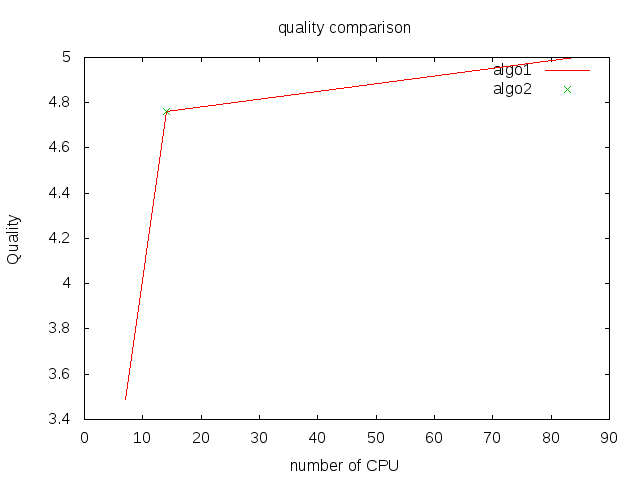
\includegraphics{03-Chapitre1/figures/comparison.png}\{fig:fig2\}

\hypertarget{deuxiuxe8me-sous-section}{%
\subsection{Deuxième sous-section}\label{deuxiuxe8me-sous-section}}

Morbi lorem. Etiam scelerisque rhoncus orci. Nunc elementum ante ac leo.
Vestibulum venenatis dictum nunc. Donec turpis est, dictum nec,
fringilla nec, cursus id, quam. In nibh orci, porttitor ut, rutrum id,
faucibus vitae, leo. Donec ut wisi. Vivamus ornare, lorem quis tristique
dapibus, nulla nisl nonummy libero, vitae luctus sem felis vel nisl.
Suspendisse lectus lacus, ultricies vitae, feugiat et, hendrerit in,
quam. Pellentesque porttitor enim at lectus. Praesent viverra laoreet
velit. Mauris neque odio, ornare id, rhoncus non, sollicitudin sed,
lectus. Phasellus et dolor. Aenean ullamcorper risus id libero.
Pellentesque ac sem eget libero aliquam tincidunt. Suspendisse neque.
Curabitur egestas neque ultrices nisl. Nulla bibendum augue et tellus.
Duis ultrices convallis est.

Lorem ipsum dolor sit amet, consectetuer adipiscing elit. Maecenas
fermentum, elit non lobortis cursus, orci velit suscipit est, id mollis
turpis mi eget orci. Ut aliquam sollicitudin metus. Mauris at sapien sed
sapien congue iaculis. Nulla lorem urna, bibendum id, laoreet iaculis,
nonummy eget, massa. Phasellus ullamcorper commodo velit. Class aptent
taciti sociosqu ad litora torquent per conubia nostra, per inceptos
hymenaeos. Phasellus est. Maecenas felis augue, gravida quis, porta
adipiscing, iaculis vitae, felis. Nullam ipsum. Nulla a sem ac leo
fringilla mattis. Phasellus egestas augue in sem. Etiam ac enim non
mauris ullamcorper scelerisque. In wisi leo, malesuada vulputate, tempor
sit amet, facilisis vel, velit. Mauris massa est, sodales placerat,
luctus id, hendrerit a, urna. Nullam eleifend pede eget odio. Duis non
erat. Nullam pellentesque.

Lorem ipsum dolor sit amet, consectetuer adipiscing elit. Maecenas
fermentum, elit non lobortis cursus, orci velit suscipit est, id mollis
turpis mi eget orci. Ut aliquam sollicitudin metus. Mauris at sapien sed
sapien congue iaculis. Nulla lorem urna, bibendum id, laoreet iaculis,
nonummy eget, massa. Phasellus ullamcorper commodo velit. Class aptent
taciti sociosqu ad litora torquent per conubia nostra, per inceptos
hymenaeos. Phasellus est. Maecenas felis augue, gravida quis, porta
adipiscing, iaculis vitae, felis. Nullam ipsum. Nulla a sem ac leo
fringilla mattis. Phasellus egestas augue in sem. Etiam ac enim non
mauris ullamcorper scelerisque. In wisi leo, malesuada vulputate, tempor
sit amet, facilisis vel, velit. Mauris massa est, sodales placerat,
luctus id, hendrerit a, urna. Nullam eleifend pede eget odio. Duis non
erat. Nullam pellentesque.

Lorem ipsum dolor sit amet, consectetuer adipiscing elit. Maecenas
fermentum, elit non lobortis cursus, orci velit suscipit est, id mollis
turpis mi eget orci. Ut aliquam sollicitudin metus. Mauris at sapien sed
sapien congue iaculis. Nulla lorem urna, bibendum id, laoreet iaculis,
nonummy eget, massa. Phasellus ullamcorper commodo velit. Class aptent
taciti sociosqu ad litora torquent per conubia nostra, per inceptos
hymenaeos. Phasellus est. Maecenas felis augue, gravida quis, porta
adipiscing, iaculis vitae, felis. Nullam ipsum. Nulla a sem ac leo
fringilla mattis. Phasellus egestas augue in sem. Etiam ac enim non
mauris ullamcorper scelerisque. In wisi leo, malesuada vulputate, tempor
sit amet, facilisis vel, velit. Mauris massa est, sodales placerat,
luctus id, hendrerit a, urna. Nullam eleifend pede eget odio. Duis non
erat. Nullam pellentesque.

Lorem ipsum dolor sit amet, consectetuer adipiscing elit. Maecenas
fermentum, elit non lobortis cursus, orci velit suscipit est, id mollis
turpis mi eget orci. Ut aliquam sollicitudin metus. Mauris at sapien sed
sapien congue iaculis. Nulla lorem urna, bibendum id, laoreet iaculis,
nonummy eget, massa. Phasellus ullamcorper commodo velit. Class aptent
taciti sociosqu ad litora torquent per conubia nostra, per inceptos
hymenaeos. Phasellus est. Maecenas felis augue, gravida quis, porta
adipiscing, iaculis vitae, felis. Nullam ipsum. Nulla a sem ac leo
fringilla mattis. Phasellus egestas augue in sem. Etiam ac enim non
mauris ullamcorper scelerisque. In wisi leo, malesuada vulputate, tempor
sit amet, facilisis vel, velit. Mauris massa est, sodales placerat,
luctus id, hendrerit a, urna. Nullam eleifend pede eget odio. Duis non
erat. Nullam pellentesque.

Lorem ipsum dolor sit amet, «\textsubscript{consectetuer}» adipiscing
elit. Maecenas fermentum, elit non lobortis cursus, orci velit suscipit
est, id mollis turpis mi eget orci. Ut aliquam sollicitudin metus.
Mauris at sapien sed sapien congue iaculis. Nulla lorem urna, bibendum
id, laoreet iaculis, nonummy eget, massa. Phasellus ullamcorper commodo
velit. Class aptent taciti sociosqu ad litora torquent per
«\textasciitilde conubia nostra\textasciitilde», per inceptos hymenaeos.
Phasellus est. Maecenas felis augue, gravida quis, porta adipiscing,
iaculis vitae, felis. Nullam ipsum. Nulla a sem ac leo fringilla mattis.
Phasellus egestas augue in sem. Etiam ac enim non mauris ullamcorper
scelerisque. In wisi leo, malesuada vulputate, tempor sit amet,
facilisis vel, velit. Mauris massa est, sodales placerat, luctus id,
hendrerit a, urna. Nullam eleifend pede eget odio. Duis non erat. Nullam
pellentesque.

Lorem ipsum dolor sit amet, «\textsubscript{consectetuer}» adipiscing
elit. Maecenas fermentum, elit non lobortis cursus, orci velit suscipit
est, id mollis turpis mi eget orci. Ut aliquam sollicitudin metus.
Mauris at sapien sed sapien congue iaculis. Nulla lorem urna, bibendum
id, laoreet iaculis, nonummy eget, massa. Phasellus ullamcorper commodo
velit. Class aptent taciti sociosqu ad litora torquent per
«\textasciitilde conubia nostra\textasciitilde», per inceptos hymenaeos.
Phasellus est. Maecenas felis augue, gravida quis, porta adipiscing,
iaculis vitae, felis. Nullam ipsum. Nulla a sem ac leo fringilla mattis.
Phasellus egestas augue in sem. Etiam ac enim non mauris ullamcorper
scelerisque. In wisi leo, malesuada vulputate, tempor sit amet,
facilisis vel, velit. Mauris massa est, sodales placerat, luctus id,
hendrerit a, urna. Nullam eleifend pede eget odio. Duis non erat. Nullam
pellentesque.

Lorem ipsum dolor sit amet, «\textsubscript{consectetuer}» adipiscing
elit. Maecenas fermentum, elit non lobortis cursus, orci velit suscipit
est, id mollis turpis mi eget orci. Ut aliquam sollicitudin metus.
Mauris at sapien sed sapien congue iaculis. Nulla lorem urna, bibendum
id, laoreet iaculis, nonummy eget, massa. Phasellus ullamcorper commodo
velit. Class aptent taciti sociosqu ad litora torquent per
«\textasciitilde conubia nostra\textasciitilde», per inceptos hymenaeos.
Phasellus est. Maecenas felis augue, gravida quis, porta adipiscing,
iaculis vitae, felis. Nullam ipsum. Nulla a sem ac leo fringilla mattis.
Phasellus egestas augue in sem. Etiam ac enim non mauris ullamcorper
scelerisque. In wisi leo, malesuada vulputate, tempor sit amet,
facilisis vel, velit. Mauris massa est, sodales placerat, luctus id,
hendrerit a, urna. Nullam eleifend pede eget odio. Duis non erat. Nullam
pellentesque.

\hypertarget{conclusion-du-premier-chapitre}{%
\section{Conclusion du premier
chapitre}\label{conclusion-du-premier-chapitre}}

Lorem ipsum dolor sit amet, consectetuer adipiscing elit. Maecenas
fermentum, elit non lobortis cursus, orci velit suscipit est, id mollis
turpis mi eget orci. Ut aliquam sollicitudin metus. Mauris at sapien sed
sapien congue iaculis. Nulla lorem urna, bibendum id, laoreet iaculis,
nonummy eget, massa. Phasellus ullamcorper commodo velit. Class aptent
taciti sociosqu ad litora torquent per conubia nostra, per inceptos
hymenaeos. Phasellus est. Maecenas felis augue, gravida quis, porta
adipiscing, iaculis vitae, felis. Nullam ipsum. Nulla a sem ac leo
fringilla mattis. Phasellus egestas augue in sem. Etiam ac enim non
mauris ullamcorper scelerisque. In wisi leo, malesuada vulputate, tempor
sit amet, facilisis vel, velit. Mauris massa est, sodales placerat,
luctus id, hendrerit a, urna. Nullam eleifend pede eget odio. Duis non
erat. Nullam pellentesque.

\clearpage
\printbibliography[heading=subbibintoc, title={Bibliographie}]
\clearemptydoublepage

\begin{refsection}

\hypertarget{from-local-seafloor-imagery-to-global-patterns-in-benthic-habitats-contribution-of-citizen-science-to-habitat-classification-across-latitudes}{%
\chapter{From local seafloor imagery to global patterns in benthic
habitats: contribution of citizen science to habitat classification
across
latitudes}\label{from-local-seafloor-imagery-to-global-patterns-in-benthic-habitats-contribution-of-citizen-science-to-habitat-classification-across-latitudes}}

\hypertarget{preambule-chapter2}{%
\section*{Préambule}\label{preambule-chapter2}}
\addcontentsline{toc}{section}{Préambule}

Le Chapitre 1 a permis de mettre en évidence deux limites majeures de
l'application des \emph{jSDM} (\emph{Joint Species Distribution Models})
pour comprendre la structure des communautés et le rôle sous-jacent des
habitats. Premièrement, que ce soit sur des données de présence/absence
ou bien d'abondance, le framework de \emph{jSDM} testé ici présentait
des performances de prédiction de la biodiversité faible, limitant
grandement ses capacités d'extrapolation spatiales et/ou temporelles.
Deuxièmement, le \emph{jSDM} étudié dans le chapitre précédent
nécessitait une importante puissance de calcul pour ajuster aux 99
espèces les plus de 16 000 paramètres nécessaires tout en leur assurant
une convergence suffisante des estimations de paramètres. Ainsi, son
application sur un jeu de données plus conséquent du \emph{Reef Life
Survey}, avec une communauté faunistique de plus de 3 000 taxons, nous a
semblé limiter son potentiel pour analyser un tel jeu de données à
l'échelle globale. De plus, dans un projet antérieur focalisé sur
l'usage des \emph{jSDM} pour l'inférence de réseau de co-occurrence des
espèces benthiques \autocite{Violet_2020}, nous avons fait face à des
incertitudes méthodologiques pour caractériser de manière robuste les
réseaux d'interactions potentiels. En effet, les réseaux reconstitués
avaient été soumis aux jugements d'un panel d'experts benthologues dont
les avis discordants n'ont pas permis de valider la véracité des
interactions identifiées. C'est pourquoi pour mieux comprendre comment
les habitats biogéniques structurent les communautés associées à
l'échelle mondiale, nous avons changé de stratégie et nous avons adopté
la méthode ``\emph{agréger, puis prédire}'' suggérée par
\textcite{Ferrier_2006}. L'objet central de ce chapitre réside dans
l'application d'une méthode de groupement peu appliquée en écologie afin
d'identifier différents états d'habitats. Le chapitre 3 complètera cette
partie d'agrégation des données par une partie prédictive.

Les particularités des données écologiques et notamment celles issues de
sciences participatives (hétérogénéité, bruit dans les données,
relations non-linéaires entre les variables d'un écosystème, etc.)
limitent la pertinence de certaines méthodes de groupement (p.~ex.
k-means, classification hiérarchique à lien simple complet, ou selon la
méthode de Ward) classiquement utilisées en écologie
(Fig.~\ref{fig:chap2chapo1}). Nous avons utilisé dans ce chapitre une
nouvelle approche de groupement pour (1) distinguer différents états
d'habitats biogéniques à partir de données issues des sciences
participatives (2) identifier des habitats iconiques, et (3)
éventuellement détecter des transitions entre différents types
d'habitats. Ce chapitre a également pour but d'étudier la distribution
de ces états d'habitats à l'échelle du globe pour valider ou non les
groupes iconiques identifiés.

\begin{figure}
\hypertarget{fig:chap2chapo1}{%
\centering
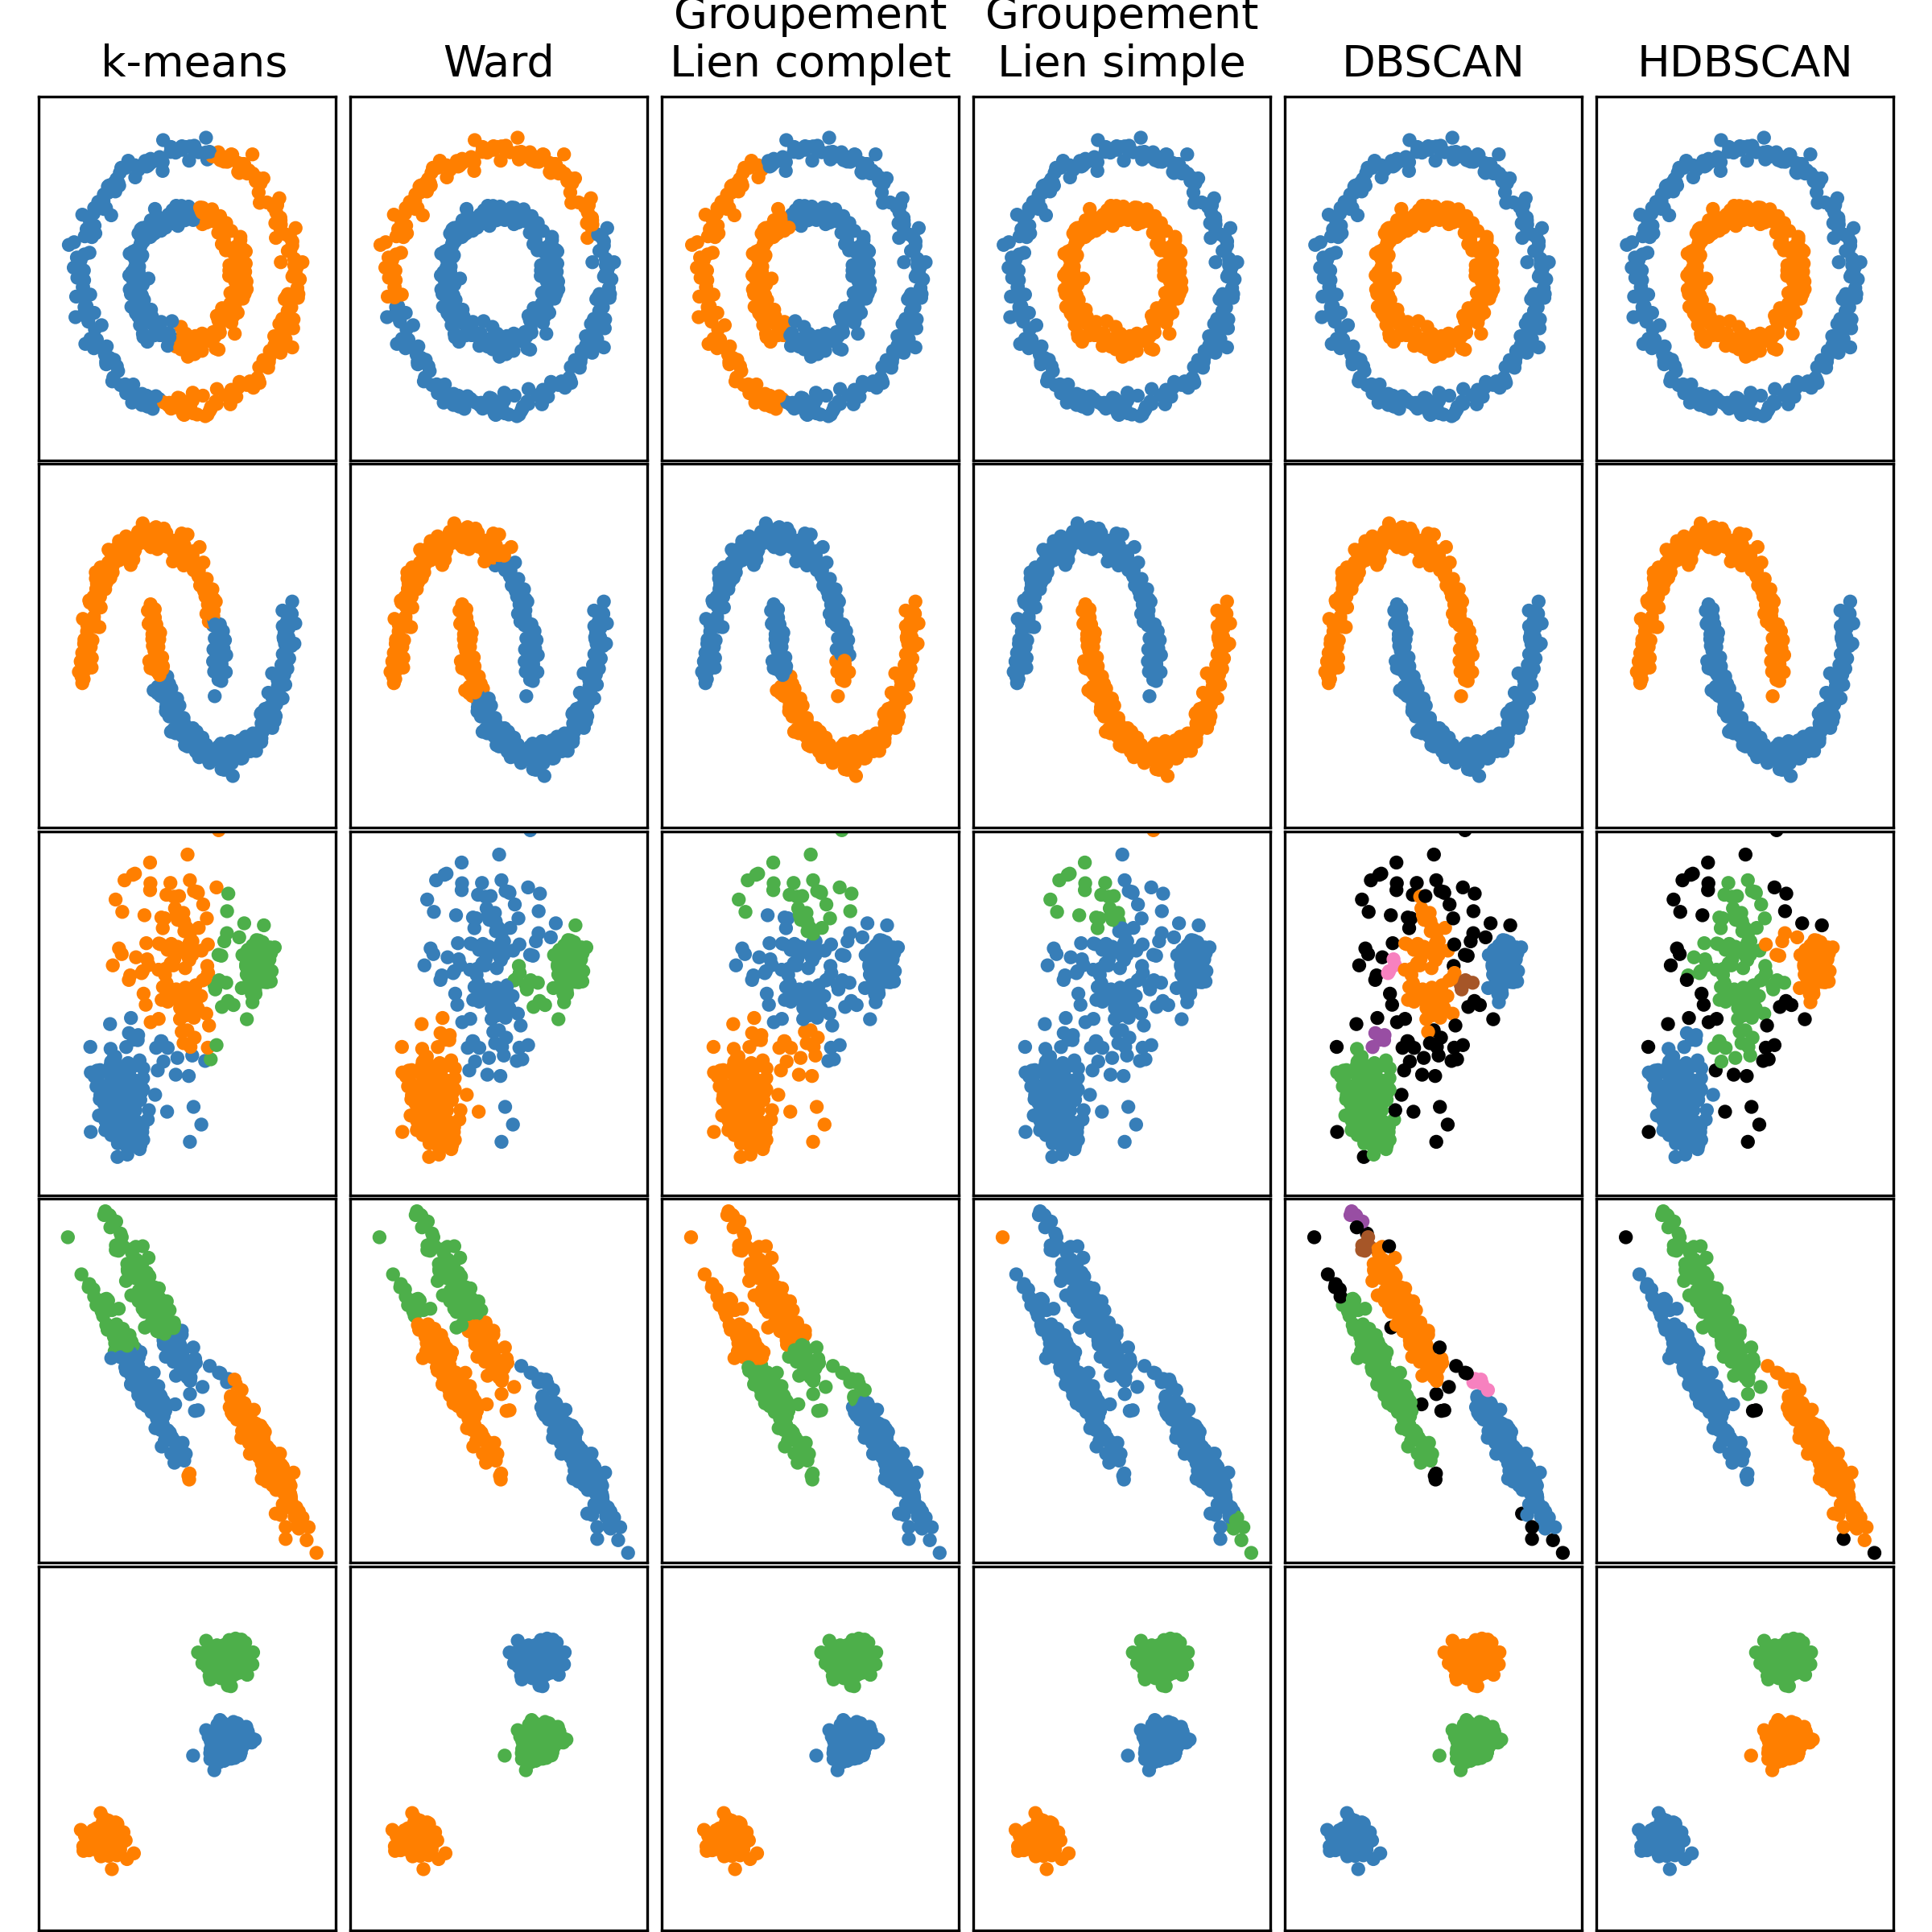
\includegraphics{03-Chapitre2/figures/synthetic_clustering_perf.png}
\caption[Comparaison de différents algorithmes de groupement utilisés en
écologie.]{Comparaison de différents algorithmes de groupement utilisés en
écologie (en colonne; à savoir k-means, Ward, groupement lien complet ou
lien simple, \mbox{DBSCAN} ou \mbox{HDBSCAN}) sur différents jeux de données simulés
en deux dimensions (en ligne). Les jeux de données des deux premières
lignes contiennent deux groupes, les trois derniers en contiennent
trois.}\label{fig:chap2chapo1}
}
\end{figure}

En amont de ce chapitre, j'ai étudié le comportement de plusieurs
combinaisons de méthodes de réductions de dimensions, ainsi que de
groupement (Fig.~\ref{fig:chap2chapo1}) ce qui a orienté le choix pour
ce Chapitre 2 vers une méthodologie qui combine un algorithme de
réduction basé sur le principe des graphes de voisinage (\emph{UMAP};
\textcite{McInnes_2020}), et une méthode de groupement basée sur la
densité (\emph{HDBSCAN}; \textcite{Moulavi_2014} ;
\textcite{McInnes2017}). En appliquant cette méthode à des données
estimant le pourcentage de couverture de différents habitats sur la base
des photoquadrats obtenus sur plus de 6 500 transects réalisés en
plongée par des volontaires du programme \emph{Reef Life Survey}, nous
avons identifié 17 états d'habitats. Certains de ces habitats
représentent des états d'habitats benthiques iconiques comme les forêts
de laminaires ou des herbiers marins, alors que d'autres représentent
des états d'habitats considérés comme dégradés, par exemple les états
dominés par la présence d'algues gazonnantes.

Ce chapitre de thèse est l'oeuvre de la collaboration de Clément Violet, Aurélien Boyé, Graham Edgar, Elizabeth Oh, Rick Stuart-Smith et de Martin Marzloff. Ce chapitre a déjà fait l'objet d'une communication orale
``\emph{Predicting reef state and regime shift risk using machine
learning and the Reef Life Surve}y'' au 13th International Temperate
Reefs Symposium 2023. Ce chapitre devrait être prochainement proposé
pour publication au journal \emph{Global Ecology and Biogeography}.

\clearpage

\hypertarget{abstract-chapt2}{%
\section{Abstract}\label{abstract-chapt2}}

\textbf{Aim:} The aim of this study was to define reef benthic habitat
states and explore their spatial and temporal variability at a global
scale using an innovative clustering pipeline.

\textbf{Location:} The study uses data on the transects surveyed on
shallow (\(<~20\)m) reef ecosystems across the globe.

\textbf{Time period:} Transects sampled between 2008 and 2021.

\textbf{Major taxa studied:} Macroalgae, sessile invertebrates,
hydrozoans, seagrass, corals.

\textbf{Methods:} Percentage cover was estimated for 24 functional
groups of sessile biota and substratum from annotated underwater
photoquadrats taken along 6,554 transects by scuba divers contributing
to the \emph{Reef Life Survey} dataset. A clustering pipeline combining
a dimension-reduction technique, \emph{Uniform Manifold Approximation
and Projection} (\emph{UMAP}), with \emph{Hierarchical Density-Based
Spatial Clustering of Applications with Noise} (\emph{HDBSCAN}), was
used to identify benthic habitat states. Spatial and temporal variation
in habitat distribution was then explored across ecoregions.

\textbf{Results:} The \emph{UMAP-HDBSCAN} pipeline identified 17
distinct clusters representing different benthic habitats and gradients
of ecological state. Certain habitat states displayed clear
biogeographic patterns, predominantly occurring in temperate regions or
tropical waters. Notably, some reefs dominated by turf algae, were
ubiquitous regardless of latitudes. Transition zones between temperate
and tropical waters emerged as spatial hotspots of habitat state
diversity. Temporal patterns revealed, changes in the proportion of
certain states showing variations over time, notably an increase in turf
algae occurrence.

\textbf{Main Conclusions:} The \emph{UMAP-HDBSCAN} clustering pipeline
effectively characterised fine-scale benthic habitat states at a global
scale, confirming known broader biogeographic patterns, including the
importance of temperate-tropical transition zones as hotspots of habitat
state diversity. This fine-scale, yet broadly-scalable habitat
classification could be applied as a standardised template for tracking
benthic habitat change across space and time at a global scale. The
\emph{UMAP-HDBSCAN} pipeline has proven to be a powerful and versatile
approach for analysing complex biological datasets and can be applied in
various ecological domains.

\clearpage

\hypertarget{intro-chapt2}{%
\section{Introduction}\label{intro-chapt2}}

Benthic habitats contribute to marine coastal ecosystems functioning and
the services they provide \autocite{Barbier_2011}. More specifically,
they contribute to shoreline protections \autocite{Barbier_2017}, carbon
sequestration \autocite{Fourqurean_2012}, support commercial fisheries
\autocite{Barbier_2017} and host diverse species and communities
\autocite{Sunday_2017}. As modifiers to abiotic substrates, foundation
species, such as kelp, seagrass, and corals engineer biogenic habitats
that contribute to specific functions of coastal ecosystems
\autocite{Elith_2009}. For instance, the tridimensional structure of
coral reefs can shelter fish assemblages from predators
\autocite{Hixon_1993}; seaweed or mussel beds can buffer environmental
conditions \autocites[ ]{Jurgens_2022}{Whitaker_2023}; and kelp forests
are both habitat and food sources for various fish and invertebrate
species \autocite{Edgar_2004}. Thus, changes in coastal benthic habitats
have direct cascading consequences on marine ecosystem structure,
functioning and services.

Being hotspots of human activity, coastal ecosystems can be adversely
affected by multiple anthropogenic stressors \autocites[
]{Bowler_2020}{Halpern_2019}. Global climate change can also lead to
fast changes in coastal abiotic conditions \autocites[
]{Burrows_2014}{Bowler_2020}. The impact of these multiple stressors on
benthic communities and ecosystems are mostly mediated by the response
of biogenic habitats like kelp, seagrass, or coral \autocites[
]{Harley_2006}{Rocha_2015b}. For example, in the vicinity of urban
areas, eutrophication can induce the replacement of kelp forests by turf
algae \autocites[ ]{Filbee-Dexter_2018}{Pessarrodona_2021}, marine
heatwaves can lead to coral bleaching, and their intensification in
magnitude and frequency can induce long-term decline in tropical coral
reefs \autocite{Bellwood_2004}, and overfishing of herbivorous fish in
these reefs can lead to the overgrowth of macroalgae on top of coral
reefs \autocite{Hughes_2007}. Hence, habitat changes are amongst the
greatest symptoms of anthropogenic impacts on shallow marine systems,
with large consequences for marine biodiversity \autocite{Rocha_2015a}.
As anthropogenic stressors on marine ecosystems tend to increase and
diversify \autocite{Halpern_2019}, habitat changes will likely become
more frequent in the future at a global scale \autocite{Conversi_2015}.
Yet, both the drivers of habitat change and its consequence on
biodiversity remain largely understudied in marine ecosystems
\autocite{Mazor_2018}.

Detecting and anticipating future habitat changes in benthic ecosystems
requires a thorough understanding of the current state and distribution
of benthic habitats and characterising of underlying drivers across
multiple scales. Currently, detailed knowledge of habitat distribution
is mostly local, i.e.~at scales ranging from study sites (10 m - 100 m)
or bay (100 m - 10 km) up to regions (10 km - 100 km) (e.g.
\textcite{Robert_2015} ; \textcite{Wicaksono_2019}), for instance using
remote sensing, acoustic surveys, or rather local monitoring of abiotic
conditions and communities \autocite{Costello_2009}. At larger scales,
habitat distribution maps are largely based on physical,
geomorphological and biogeochemical ocean properties (e.g.
\textcite{Brown_2011} ; \textcite{Lecours_2015} ;
\textcite{Sonnewald_2020}). At such scales, habitat maps either
disregard biogenic habitats or remain species-specific. Indeed, studies
that focus on biogenic habitat distribution tend to consider specific
habitat-formers independently \autocites[ ]{Assis_2020}{McKenzie_2020}
and rarely provide information on community composition. Large-scale
seafloor habitat maps of either abiotic, or biogenic features also tend
to integrate data over large timescales (e.g.~decades). Their aim is
rather to provide a static picture of the potential distribution of
these habitats than to infer changes in habitat states and distribution.
Knowledge of benthic habitat changes thus remains highly regional (e.g.
\textcite{Cattano_2020}). In that context several global studies have
collated heterogeneous regional monitoring data to document changes in
emblematic habitat-formers, such as seagrass spp. \autocites[
]{Waycott_2009}{Dunic_2021}, kelp beds \autocites[
]{Krumhansl_2016}{Filbee-Dexter_2018} or coral reefs
\autocite{Eddy_2021}. Yet, these independent studies on specific
habitat-formers are not sufficient to gain a comprehensive understanding
of how the seafloor habitat mosaic has changed over the last decade at a
global scale and how it is now changing in the face of anthropogenic
pressures. Our understanding of current changes in seafloor habitat
mosaic is impeded by the lack of large-scale, standardised, data-driven
definition and maps of benthic habitat and their potential states.

Identifying changes in benthic habitat states through space and time
requires a standardised workflow from data collection through to
systematic statistical discrimination between habitat states. In this
study, we aim to develop a data-driven pipeline that distinguishes
different iconic benthic habitats observed spatially, and apply this to
characterise stepwise changes in habitat ecological states through time.
Because scientific monitoring programmes are often expensive
\autocite{Edgar_2016} and restricted in their spatial and/or temporal
coverage \autocite{Rhodes_2015}, participatory science programmes have
emerged as valuable means to increase monitoring programme coverage and
resolution. In this study, we leverage the benefits of a citizen science
program to characterise benthic habitat states at the global scale and
overcome the limitations of traditional scientific programs. The
\emph{Reef Life Survey} (\emph{RLS}) relies on standardised diver-based
50-metre-long transects to estimate fish and invertebrate species
abundance as well as image-based percentage cover of coastal benthic
habitats \autocite{Edgar_2014b}. Estimates of habitat percentage cover
have already proven useful for defining habitat states at a regional
scale through the use of unsupervised machine learning techniques
\autocites[ ]{Cresswell_2017}{PelletierD_2020}. However, the methods
proposed in these previous studies come with a number of limitations
when upscaling these approaches at a global scale. In particular, the
occurrence and abundance of habitat-forming species are expected to show
non-linear responses to environmental changes \autocite{Oksanen_2002},
especially across large environmental gradients. Still, the clustering
algorithm used for \textcite{Cresswell_2017} and
\textcite{PelletierD_2020} are not adapted to take into account the
non-linear nature of the dominance patterns between different
habitat-forming species.

Hence, we applied a new workflow, combining two algorithms to overcome
these challenges: (1) \emph{Uniform Manifold Approximation and
Projection} (\emph{UMAP}) a novel dimension reduction technique
preserving complex nonlinear structures and patterns
\autocite{McInnes_2020}, (2) and the \emph{Hierarchical Density-Based
Spatial Clustering of Applications with Noise algorithm}
(\emph{HDBSCAN}) that can identify clusters of varying shapes and sizes
while filtering out outlier noise \autocites[
]{Campello_2013}{McInnes2017}. While previous ecological studies have
successfully applied both \emph{UMAP} for dimension reduction
\autocite{Milosevic_2022} and \emph{HDBSCAN} for food web classification
\autocite{Ohlsson_2020}, our study represents a novel application to
coastal marine habitats. We interpret classification results by
combining the latest \emph{SHapley Additive exPlanations} (\emph{SHAP})
\autocite{Lundberg_2017} framework with visual inspections of
photoquadrats associated with the most representative transects of the
different clusters.

Therefore, the aim of this study is to characterise coastal benthic
habitat states using a \emph{UMAP-HDBSCAN} pipeline on the \emph{RLS}
habitat dataset. Using this pipeline, we identify and classify benthic
habitat states at a global scale and characterise their spatial and
temporal variability across biogeographical gradients as well as within
bioregions.

\clearpage

\hypertarget{mat-met-chapt2}{%
\section{Materials \& Methods}\label{mat-met-chapt2}}

We used a \emph{UMAP-HDBSCAN} pipeline to cluster the global \emph{RLS}
benthic habitat dataset. In the following sections, we sequentially
describe : (1) the data used in this study, (2) the clustering pipeline,
(3) the interpretation of the identified clusters.

\hypertarget{data}{%
\subsection{Data}\label{data}}

\hypertarget{reef-life-survey-photoquadrat-dataset}{%
\subsection{\texorpdfstring{\emph{Reef Life Survey} photoquadrat
dataset}{Reef Life Survey photoquadrat dataset}}\label{reef-life-survey-photoquadrat-dataset}}

The \emph{RLS} (\url{http://www.reeflifesurvey.com/}) is a hybrid
citizen science/professional researcher program monitoring reef
communities around the world using scuba-diving visual census. Details
about the survey methods, including protocols, diver training, data
quality assurance and data management, are covered by
\textcite{Edgar_2014}. Here, we used estimates of relative cover of
benthic habitats derived from in situ digital photoquadrats: along
standardised 50 m transect, 20 photoquadrats, which each approximately
covers 0.3 m × 0.3 m, are collected every 2.5 m \autocite{Edgar_2020}.
Images are then annotated using point counts on the \emph{Squidle+}
(\url{https://squidle.org/}) platform to estimate the percentage covers
of about 50 substratum types and functional groups, based on the
\emph{CATAMI} benthic imagery classification scheme
(\textcite{Althaus_2015} ; for further details, see
\textcite{Edgar_2020}). Based on \emph{RLS} specialists' expertise,
these 50 original benthic habitat categories (see Appendix A, Table 1 in
Supporting Informations) were grouped into 24 broader categories
(Table~\ref{tbl:chap2table1}) that more consistently capture the range
of dominant coastal substratum available along \emph{RLS} transects at
the global scale.

We extracted the \emph{RLS} photoquadrat dataset on 24 January 2023.
From the original 8,154 transects, we removed partially scored
transects. For transects annotated multiple times on \emph{Squidle+}
across various research projects, mean percentage cover estimates were
considered. After fully curating the dataset, the photoquadrat dataset
consisted of 6,554 transects across 2,249 sites over the world. All
subsequent analyses were performed at the transect level to consider
local-scale variation in the state of benthic habitats.

\hypertarget{tbl:chap2table1}{}
\begin{longtable}[]{@{}
  >{\centering\arraybackslash}p{(\columnwidth - 2\tabcolsep) * \real{0.2614}}
  >{\raggedright\arraybackslash}p{(\columnwidth - 2\tabcolsep) * \real{0.7386}}@{}}
\caption[Description of the 24 categories used in
this study to overall capture the diversity of habitat types sampled by
\emph{Reef Life Surveys} worldwide.]{\label{tbl:chap2table1}Description of the 24 categories used in
this study to overall capture the diversity of habitat types sampled by
\emph{Reef Life Surveys} worldwide. The 50 original \emph{RLS}
categories were lumped into these 24 categories that represent
ecologically-consistent groups associated with different levels of
structural complexity.}\tabularnewline
\toprule\noalign{}
\begin{minipage}[b]{\linewidth}\centering
\textbf{Habitat Categories}
\end{minipage} & \begin{minipage}[b]{\linewidth}\raggedright
\textbf{Description}
\end{minipage} \\
\midrule\noalign{}
\endfirsthead
\toprule\noalign{}
\begin{minipage}[b]{\linewidth}\centering
\textbf{Habitat Categories}
\end{minipage} & \begin{minipage}[b]{\linewidth}\raggedright
\textbf{Description}
\end{minipage} \\
\midrule\noalign{}
\endhead
\bottomrule\noalign{}
\endlastfoot
\multicolumn{2}{@{}c@{}}{%
\emph{Erect algae}}\\\hline

Large canopy forming algae & Large overstorey algae forming a canopy,
including kelps or large fucoids \\
Bushy Fucoid like & Robust vertical leaf-liked shaped brown algae \\
Other Brown algae & Thick or thin-sheet like vertical algae \\
Red algae & Foliose vertical red algae \\
Green algae & Thin-sheet like, thick, or ribbon-like, vertical growth
algae \\\hline
\multicolumn{2}{@{}c@{}}{%
\emph{Erect calcareous algae}} \\\hline
Geniculate coralline algae & Red vertical calcified segmented algae \\
Green calcified algae & Small calcified green algae \\
\hline
\multicolumn{2}{@{}c@{}}{%
\emph{Encrusting algae}} \\\hline
Crustose coralline algae & Red algae forming a small calcified crust
over hard substrate \\
Encrusting algae & ~Algae forming a leathery crust over a substrate \\
\hline
\multicolumn{2}{@{}c@{}}{%
\emph{Mat-forming Algae}} \\\hline
Filamentous algae & Filamentous algae, epiphyte or rock-attached \\
Turf algae & Fine and mat-forming filamentous algae growing on hard
substrate \\
\hline
\multicolumn{2}{@{}c@{}}{%
\emph{Plant}} \\\hline
Seagrass & Vertical ribbon-like marine plant \\
\hline
\multicolumn{2}{@{}c@{}}{%
\emph{Sessile invertebrates}} \\\hline
Encrusting corals & Stony corals forming a crust over hard substrate \\
Branching coral & Branching coral forming large colonies \\
Foliose/Plate corals & Stony corals forming tabular or foliaceous
colonies \\
Massive corals & Stony corals characterised by large, ball- or
boulder-shaped colonies with a compact structure \\
Large-polyp stony corals & Large lobed stony coral, usually
free-living \\
Soft corals and gorgonians & Soft coral or gorgonian in the sub-class
Octocorallia \\
Calcareous hydrocorals and octocorals & Branching or foliaceous
coral-like \\
Other sessile invertebrates & Habitat-forming sessile invertebrates
(e.g.~sponges, ascidians, bryozoans or molluscs) excluding corals \\
\hline
\multicolumn{2}{@{}c@{}}{%
\emph{Seabed Materials}} \\
\hline
Dead coral & Dead attached coral skeleton \\
Bare rocky substrate & Bare rock \\
Unconsolidated substrate & Gravel, shell, coral rubble \\
Sand & Sand and fine sediments \\
\end{longtable}

\clearpage

\hypertarget{clustering-pipeline}{%
\section{Clustering pipeline}\label{clustering-pipeline}}

To account for non-linear, high-dimensional and complex nature of the
ecological data, we combined a graph theoretical dimension reduction
technique and a density-based classification technique, which has
successfully identified ecoprovinces using biogeochemical ocean data at
a global scale \autocite{Sonnewald_2020}. Among the set of methods
available, we have chosen the \emph{UMAP} algorithm
\autocite{McInnes_2020} and the \emph{HDBSCAN} algorithm \autocites[
]{Campello_2013}{McInnes2017} for dimension reduction and clustering,
respectively.

\hypertarget{dimension-reduction---umap}{%
\subsection{\texorpdfstring{Dimension reduction -
\emph{UMAP}}{Dimension reduction - UMAP}}\label{dimension-reduction---umap}}

The \emph{UMAP} algorithm is a non-linear reduction technique
\autocite{McInnes_2020}. Unlike more traditional methods applied in
ecology such as \emph{Principal Component Analysis} (\emph{PCA}),
\emph{UMAP} preserves both the local structure (preserving the distance
between neighbouring points) and the global structure (preserving the
distances between the most different points) of the raw dataset
\autocite{McInnes_2020}. These two key properties have been proven
useful for reducing the dimension of complex genomic
\autocite{Dorrity_2020}, or ecological \autocite{Milosevic_2022} data
prior to clustering. \emph{UMAP} reduces the dimensionality of a dataset
by first creating a high-dimensional graph that connects each data point
to its k-nearest neighbours. Then, \emph{UMAP} produces a
low-dimensional representation of this high-dimensional graph that
reflects the original dataset \autocite{McInnes_2020}. \emph{UMAP}
requires a distance matrix to construct the initial k-nearest-neighbour
graph. Here, we applied the Chord transformation to standardise
percentage cover data as relative cover per transect before computing
euclidean distances between transects \autocite{Legendre_2001}. In
addition to the choice of a suitable distance metric, two \emph{UMAP}
hyperparameters can influence dimension reduction. The first one is the
number of neighbours \emph{n\_neighbors} to consider when creating the
k-nearest neighbour graph. Low \emph{n\_neighbors} values will allow the
embedding to preserve more of the local structure of the original
distance matrix and larger ones will preserve more of the global
structure \autocite{McInnes_2020}. The second parameter is
\emph{min\_dist}, which controls the packing density at which
\emph{UMAP} is allowed to clump similar points in the reduced
dimensional space. A high value of \emph{min\_dist} will tend to
preserve the overall topological structure of the data, while a low
value allows \emph{UMAP} to clump closely similar points on the
embedding. The value of \emph{n\_neighbors} has been tuned in this
study, while the value of \emph{min\_dist} has been set to 0.0, since
this value allows densification of the low-dimensional representation of
the dataset, which is important before using a density-based
classification algorithm \autocite{Vermeulen_2021}.

\hypertarget{clustering---hdbscan}{%
\subsection{\texorpdfstring{Clustering -
\emph{HDBSCAN}}{Clustering - HDBSCAN}}\label{clustering---hdbscan}}

After embedding our data into a two-dimensional space, we clustered the
generated projections of the data with the unsupervised hierarchical
density-based clustering \emph{HDBSCAN} algorithm that can provide both
hard (i.e.~samples are exclusively assigned to a single cluster) and
soft (i.e.~samples are assigned probabilities of belonging to the
different clusters) clustering solutions. In addition to identifying
clusters of various shapes and density from a dendrogram, this algorithm
comes with several advantages in ecology both in terms of classification
and interpretation:it can exclude noisy observations, which do not get
assigned to any clusters, and can also highlight most representative
members of each cluster \autocites[ ]{Campello_2013}{McInnes2017}.

The \emph{HDBSCAN} clustering algorithm involves a few core steps.
First, it computes the core distance for the k-nearest neighbours for
all points in the dataset. Then, it computes the extended minimum
spanning tree from a weighted graph, where the edges are weighted by the
distance between two points while taking into account the density of
points around them. Then, \emph{HDBSCAN} builds a hierarchy from the
extended minimum spanning tree by cutting it at different levels of
density. If the cut results in the creation of clusters smaller than the
minimal number of observations set by the user
\emph{min\_cluster\_size}, all points members of these clusters are
declared as noise by the algorithm. The algorithm stops when it declares
all points as noise and returns to the user a tree-like structure where
each node corresponds to a cluster varying in shape and density
\autocites[ ]{Campello_2013}{McInnes2017}. In this study, we tuned only
one parameter for \emph{HDBSCAN}: the \emph{minimum\_cluster\_size},
controlling for the minimal number of observations required to form a
cluster and used the default parameters otherwise.

\hypertarget{evaluation-of-the-clustering-output}{%
\subsection{Evaluation of the clustering
output}\label{evaluation-of-the-clustering-output}}

For this pipeline, we search the best combination of hyperparameters for
both \emph{UMAP} (\emph{n\_neighbors}) and \emph{HDBSCAN}
(\emph{minimum\_cluster\_size}) using a complete grid search. We
exhaustively explored results sensitivity to the two hyperparameters
from 10 to 500 resulting in 241,081 models evaluated. The best
combination was found by optimising both the quality of the embedding
and the clustering, using two criteria. The \emph{UMAP} embedding was
evaluated with the trustworthiness metric \autocite{Venna_2001}, ranging
from 0 to 1 (the higher the index the more the local structure of the
original data is preserved). The quality of the clustering was evaluated
with the \emph{DBCV}, which measures both compactness within and
separations between clusters \autocite{Moulavi_2014}. The \emph{DBCV}
index, which ranges between -1 and 1, is appropriate to asses the
quality clusters with varying shapes and densities
\autocite{Moulavi_2014}.

A previous fine-scale analysis by \textcite{Cresswell_2017} on a
regional subset of this dataset yielded nine groups of habitats. We
expected to found at least that many groups at the global scale and thus
restrained our search of the best hyperparameter combinations to the
solution yielding at least the same number of cluster than
\textcite{Cresswell_2017}. Among these solutions, we select the best
combination of hyperparameter (\emph{n\_neighbors} = 400 ;
\emph{min\_cluster\_size} = 74) yielding the best performance in terms
of both their trustworthiness and \emph{DBCV} scores, while having the
maximal number of clusters for a finer granularity.

\hypertarget{interpretation-of-the-clusters}{%
\subsection{Interpretation of the
clusters}\label{interpretation-of-the-clusters}}

To interpret individual clusters identified with \emph{UMAP-HDBSCAN}, we
computed the mean percentage cover of each habitat in each cluster. Then
we used the \emph{SHAP} framework to further explore how potential
nonlinear interactions between variables may determine clustering
outcomes \autocite{Lundberg_2017}. Because of the computational cost of
applying \emph{SHAP} to our complete pipeline, we used a classification
tree \autocite{Breiman_1984} to approximate the clustering pipeline
(i.e.~predict label cluster membership based on the raw percentage cover
variables) before applying the \emph{SHAP} framework
\autocite{Lundberg_2017}. In order to train our classification tree, we
used a stratified train-test split to ensure that the relative frequency
of each cluster label is preserved in the train and test fold. The
training and the test sets contain 80\% and 20\% of the data,
respectively. Then, we used a minimal cost-complexity pruning algorithm
to avoid overfitting of our classification tree \autocite{Breiman_1984}
and estimated classification error rates using the F1-score
\autocite{vanRijsbergen_1979}. The classification error rates were
satisfactory, F1-score of 0.99 and 0.94 on the train and test sets
respectively. Based on the \emph{SHAP} values that estimate the
influence of each variable to cluster definition, we examined potential
interactions between the two most characteristic variables for each
cluster by performing a piecewise linear interpolation of the
\emph{SHAP} values. Finally, we completed interpretation by extracting
the photoquadrats for these transects considered by \emph{HDBSCAN} as
the most representative members of their cluster.

\hypertarget{spatio-temporal-distribution-of-benthic-habitat-states}{%
\subsection{Spatio-temporal distribution of benthic habitat
states}\label{spatio-temporal-distribution-of-benthic-habitat-states}}

We first explored the latitudinal distribution of each cluster. We also
summarised their occurrence within each of the \emph{Marine Ecoregions
of the World} (\emph{MEOW}; \textcite{Spalding_2007}) sampled by the
\emph{RLS}. In addition to examining dominant clusters per ecoregion, we
also computed the proportion of transects classified as noise, as well
as the Gini-Simpson diversity index. We chose this diversity index
because it focuses on changes in dominance patterns, more indicative of
changes in landscapes and is more robust to low sampling issues than
other diversity indices \autocite{Lande_2000}.

We identified sites within the \emph{RLS} that had been sampled at least
twice. We split our dataset into two equal sets (corresponding to the
2008-2013 and the 2014-2021 periods) based on the median number of
transects carried out over the study period in the most surveyed
ecoregions (i.e.~where more than 30 transects were performed in each
period). As a result, only five ecoregions in South-East Australia were
analysed. We investigated temporal changes between the two periods by
comparing the proportion of habitat identified in each ecoregion, as
well as overall when pooling all five ecoregions together.

\clearpage

\hypertarget{results-chapt2}{%
\section{Results}\label{results-chapt2}}

Based on extensive exploring of hyperparameter space, both
trustworthiness score of \(0.98 \pm 0.002\) (mean \(\pm\) sd) and
\emph{DBCV} score of \(0.46 \pm 0.08\) (mean \(\pm\) sd) for solution
containning at least 9 group suggest that these solutions yield reliable
clustering of the \emph{RLS} photoquadrat dataset (Annexe B Fig. S1 in
Supporting Informations). Across these best solutions, optimal number of
clusters varied between 9 and 184 (\(22.81 \pm 18.37\); mean \(\pm\) sd)
while mean number of points classified as noise was
\(2,207.33 \pm 364.95\) (mean \(\pm\) sd). Hereafter, out of theses, we
chose to focus on the single solution yielding the highest resolution
(i.e.~the greatest number of clusters; see Fig.~\ref{fig:chap2fig1} for
a description of the habitat states uncovered), and the smaller number
of transects classified as noise (1,464 transects) possible. This
solution has a trustworthiness score of 0.98 for \emph{UMAP} and a
\emph{DBCV} score of 0.60 for \emph{HDBSCAN}. The number of clusters
identified by this set of hyperparameters is 17
(Fig.~\ref{fig:chap2fig1}).

\begin{figure}
\hypertarget{fig:chap2fig1}{%
\centering
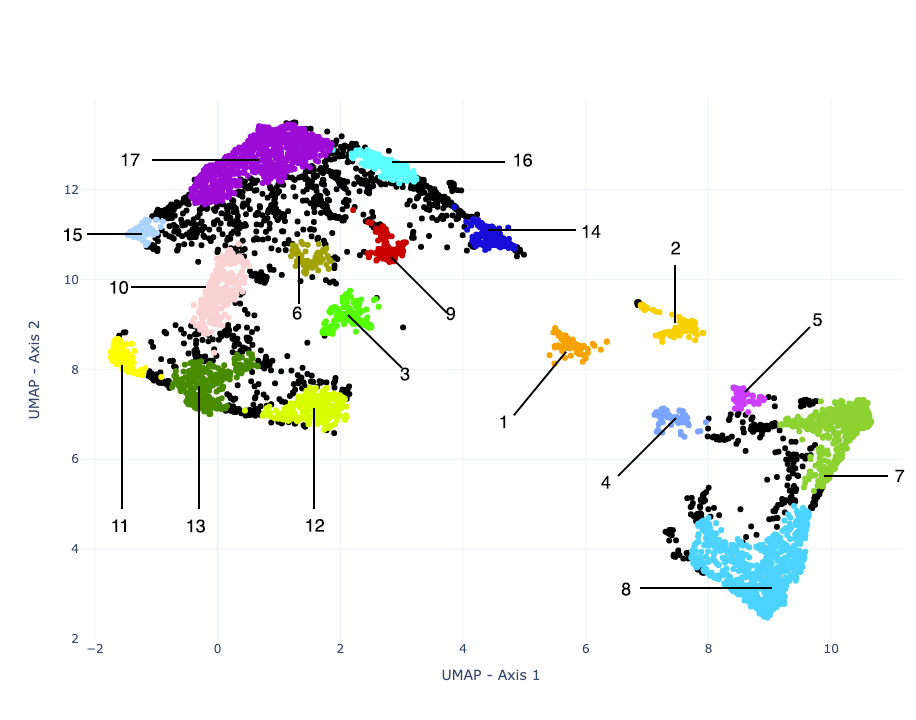
\includegraphics{03-Chapitre2/figures/fig1.png}
\caption[Two-dimensional \emph{UMAP} embedding of the benthic cover data
of the 6,554 \emph{RLS} transects.]{Two-dimensional \emph{UMAP} embedding of the benthic cover data
of the 6,554 \emph{RLS} transects. Each point corresponds to an \emph{RLS}
transect, coloured according to membership for the selected
\emph{UMAP-HDBSCAN} pipeline. Black dots represent points classified as
noise (n=1464). The 17 clusters can be interpreted as follows (see
Fig.~\ref{fig:chap2fig2} and S20-36): 1. \emph{Foliose brown algae}
(n=148) 2. \emph{Filamentous algae} (n=208) 3. \emph{Other Sessile
invertebrates} (n=185) 4. \emph{Foliose red algae} (n=123) 5.
\emph{Seagrass} (n=83) 6. \emph{Soft coral and gorgonians} (n=98) 7.
\emph{Bushy fucoids} (n=577) 8. \emph{Canopy forming algae} (n=894) 9.
\emph{Unconsolidated substrate} (n=151) 10. \emph{Crustose coralline and
turf algae} (n=286) 11. \emph{Green calcified algae} (n=166) 12.
\emph{Bare substrates} (n=329) 13. \emph{Crustose coralline algae}
(n=409) 14. \emph{Sand} (n=220) 15. \emph{Branching coral} (n=110) 16.
\emph{Turf and sand} (n=207) 17. \emph{Turf algae}
(n=897)}\label{fig:chap2fig1}
}
\end{figure}

The 17 clusters identified can be summarised hereafter according to four
broad groups (Fig.~\ref{fig:chap2fig3}, \ref{fig:chap2fig3}, see Fig S2-S19 for their
distribution on the globe and S20-36 for their interpretation with
\emph{SHAP} framework in Supporting Informations): (1) temperate
habitats, (2) subtropical and tropical habitats, (3) broadly-distributed
habitats and (4) opportunistic habitats (i.e.~habitats with documented
ecological dysfunctions - and therefore often habitats under strong
anthropogenic influence, characterised by the presence of filamentous
algal species or turf).

Transects within temperate regions can be classified according to five
major clusters associated with contrasted dominance of sessile
invertebrates, foliose red algae, seagrass, bushy foliose algae and
canopy-forming algae, as follows: cluster 3 is dominated by at least
30\% and on average 42\% of sessile invertebrates. Cluster 4 is
dominated by at least 40\% coverage of foliose red algae. Cluster 5 is
dominated by at least 30\% and on average 40\% seagrass. Cluster 7 is
dominated by at least 20\% coverage and an average of 56\% fucoid bushy
algae and an absence of canopy forming algae. Cluster 8 is characterised
by a cover of at least 20\% and an average of 55\% of canopy forming
algae with an absence of fucoid bushy algae.

Three clusters correspond to tropical and sub-tropical habitat types.
Cluster 6 which is characterised by at least 30\% and on average 37\% of
soft corals and gorgonians. Cluster 11 is composed of 20\% coverage and
an average of 35\% green calcified algae. Finally cluster 15 is composed
of at least 35\% and on average 55\% branching coral. Interestingly,
this is the only group of corals identified in the dataset given the
four categories of colony-forming corals.

Five clusters correspond to broadly-distributed habitats that can occur
across both temperate and tropical latitudes. Cluster 1 is dominated by
at least 30\% and on average 46\% brown foliose algae. Cluster 9 is
dominated by the presence of at least 30\% and on average 41\%
unconsolidated substrate. Cluster 12 has at least 30\% and on average
42\% bare substrate. Cluster 13 is characterised by 40\% and on average
51\% of crustose coralline algae with an absence of turf algae. Cluster
14 has at least 30\% and an average of 53\% sand without turf algae.

Finally, four clusters correspond to opportunistic habitats. Cluster 2
is in that respect dominated by at least 30\% coverage and an average of
39\% filamentous algae. Clusters 10, 11 and 17 are all dominated by turf
algae. Cluster 10 is composed of at least 30\% and on average 39\% of
turf algae and at least 20\% and on average 28\% of crustose coralline
algae. Cluster 16 is characterised by the presence of at least 30\% and
on average 48\% turf algae and a minimum coverage of 20\% and on average
26\% sand. Cluster 17 is composed of at least 40\% and on average 60\%
turf algae with an absence of crustose coralline.

\begin{figure}
\hypertarget{fig:chap2fig2}{%
\centering
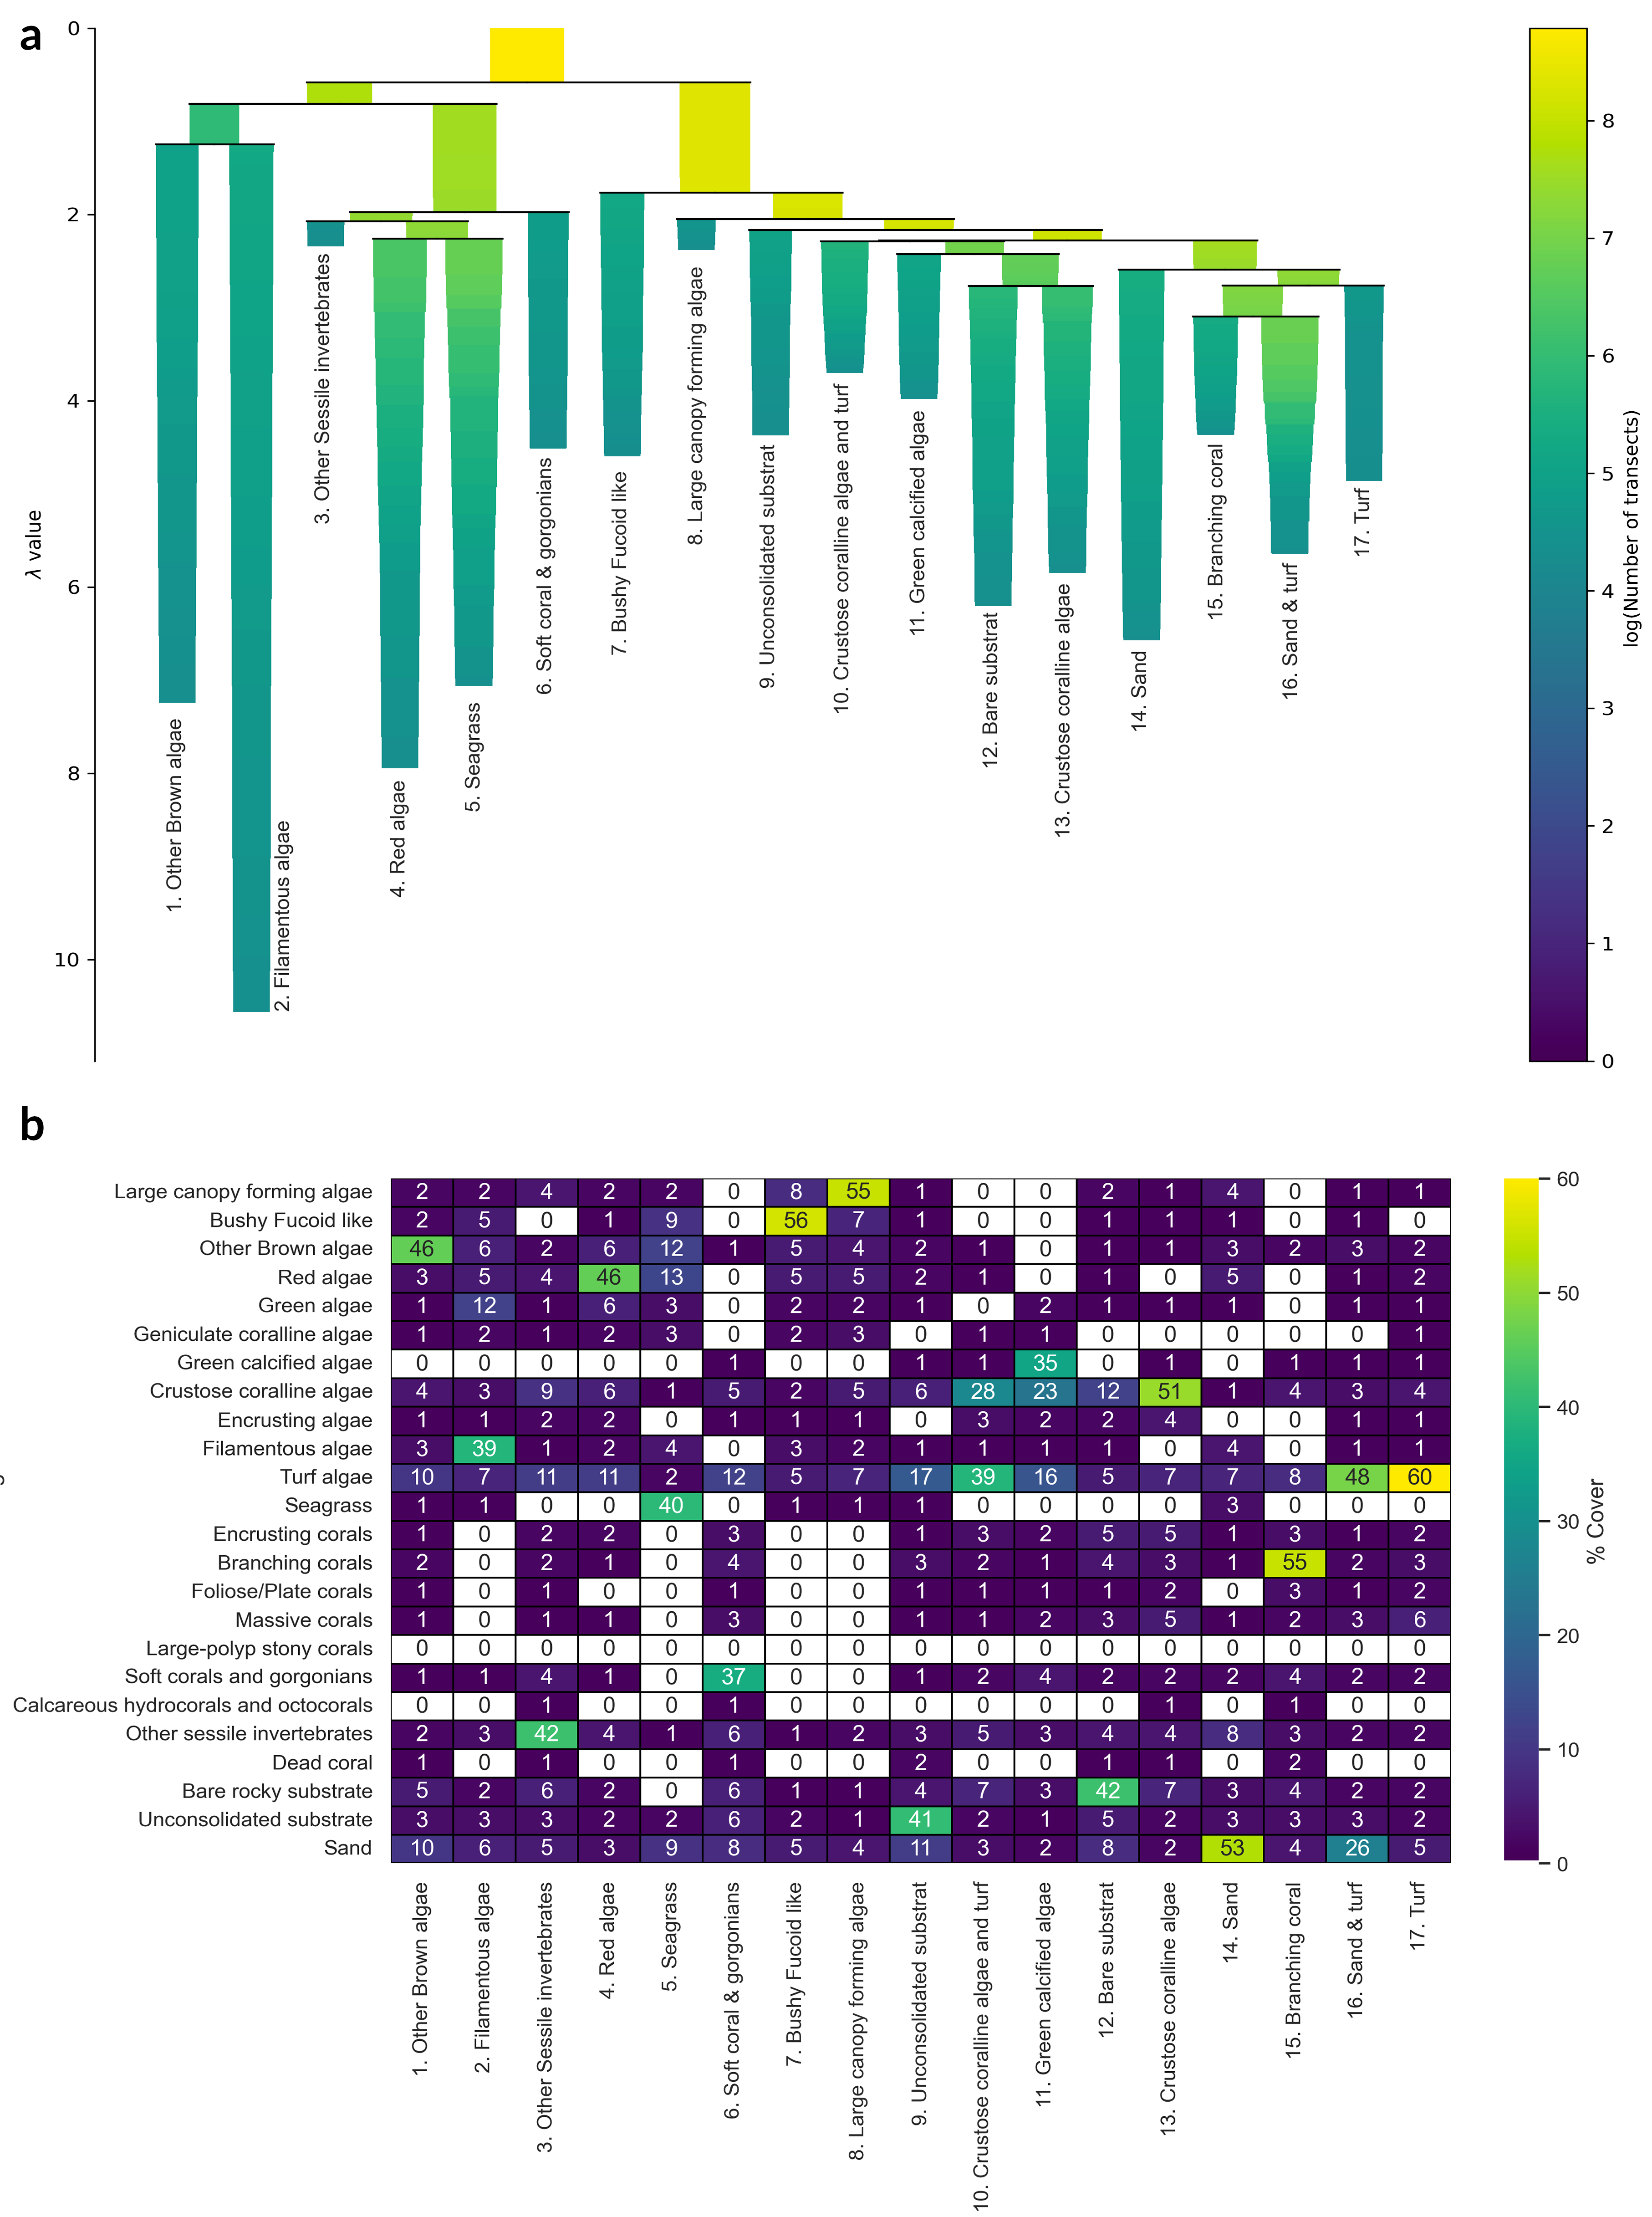
\includegraphics{03-Chapitre2/figures/fig2.png}
\caption[a. \emph{HDBSCAN} condensed clustering tree of the \emph{UMAP}
2D embedding b. Heatmap of the mean substrate coverage for each cluster identified 
by the \emph{UMAP-HDBSCAN} pipeline.]{a. \emph{HDBSCAN} condensed clustering tree of the \emph{UMAP}
2D embedding b. Heatmap of the mean substrate coverage (rounded to the
nearest integer) for each cluster identified by the \emph{UMAP-HDBSCAN}
pipeline.}\label{fig:chap2fig2}
}
\end{figure}

The clusters identified by the \emph{UMAP-HDBSCAN} pipeline show a
marked latitudinal gradient (Fig.~\ref{fig:chap2fig3}). \emph{Red
algae}, \emph{filamentous algae}, \emph{fucoids}, \emph{canopy-forming
algae} and \emph{seagrass} are essentially distributed overall in the
temperate zones across latitudes higher than 25°
(Fig.~\ref{fig:chap2fig3}). Conversely, 4 habitat states, namely
\emph{soft corals and gorgonians}, \emph{green calcified algae},
\emph{sand and turf} and \emph{branching coral} essentially occur in
tropical latitudes (lower than 25°) (Fig.~\ref{fig:chap2fig3}). However,
some groups are relatively ubiquitous across all surveyed latitudes such
as those associated with transects classified as \emph{noise},
\emph{bare} and \emph{unconsolidated substrate}, \emph{brown algae},
\emph{crustose coralline algae} with and without \emph{turf algae} and
\emph{turf algae} (Fig.~\ref{fig:chap2fig3}).

\begin{figure}
\hypertarget{fig:chap2fig3}{%
\centering
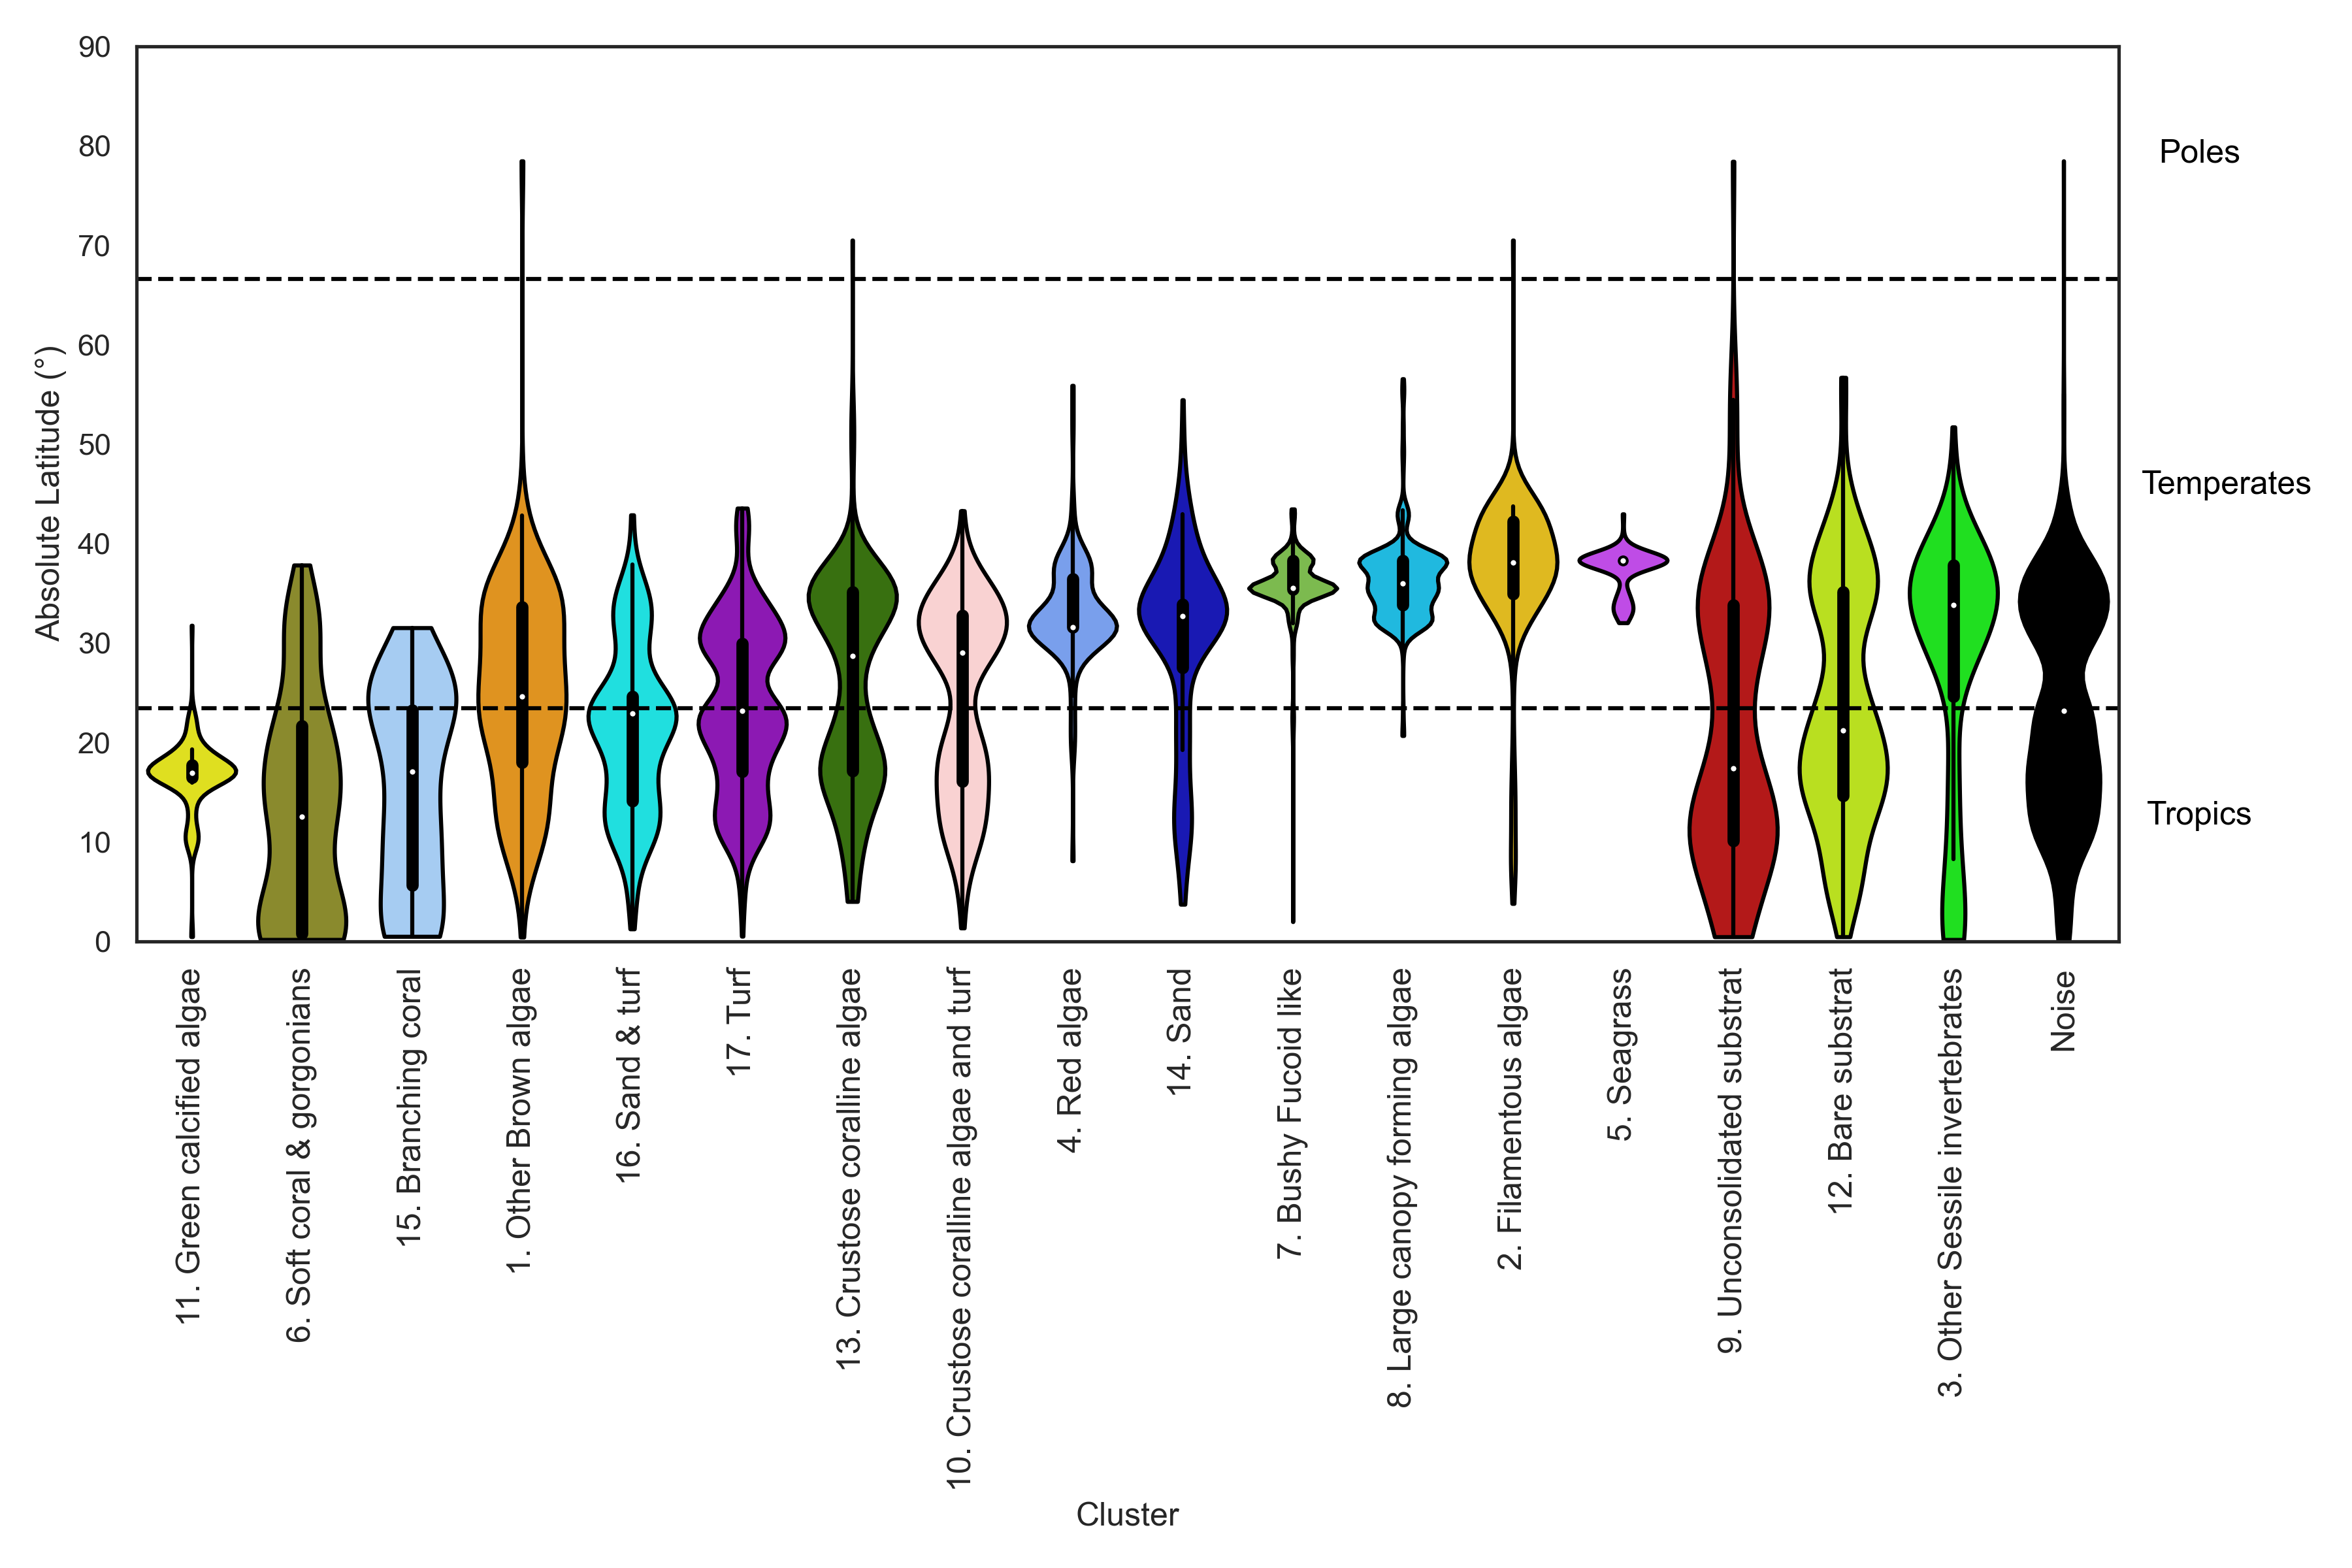
\includegraphics{03-Chapitre2/figures/fig3a.png}
\caption{Violin plot of the absolute latitudinal distribution of the
different hard cluster solutions.}\label{fig:chap2fig3}
}
\end{figure}

The spatial distribution of transects sampled by \emph{RLS} volunteers
is particularly concentrated in Australia (Fig.~\ref{fig:chap2fig4} a).
However, other areas such as the Caribbean, the Azores, and French
Polynesia have also been extensively surveyed with more than 50
transects (Fig.~\ref{fig:chap2fig4} a). Globally, three habitat types
dominate in terms of occurrences across all surveyed ecoregions, namely
\emph{bare substrate} (n = 20), \emph{turf} (n = 17), and
\emph{canopy-forming algae} (n = 11). These three habitat types dominate
in 37\% of the ecoregions sampled by the \emph{RLS}
(Fig.~\ref{fig:chap2fig4} b). Two habitat types identified by the
\emph{UMAP-HDBSCAN} pipeline, \emph{seagrass} and \emph{red algae}, are
not dominant in any of the world's ecoregions. The patterns of dominance
of the different clusters also vary along the latitudinal gradient
(Fig.~\ref{fig:chap2fig4} b), in line with the latitudinal distribution
of each cluster (Fig.~\ref{fig:chap2fig3}). These latitudinal variations
of dominance are visible both at a global scale, but also along certain
regions. For instance, a decrease in prevalence of sites in the
canopy-forming algae cluster accompanies an increase in sites in the
turf cluster along the coastline from southern to northern Australia
(Fig.~\ref{fig:chap2fig4} b).

The proportion of noisy transects is highly heterogeneous across the
globe (Fig.~\ref{fig:chap2fig4} c). Noisy transects represent 23\% of
all transects analysed, but are present in some areas more than in
others. For example, in the Southern California Bight (western USA),
Bight of Sofala/Swamp Coast (Eastern Africa), the Seychelles, and in
Three Kings-North Cape (northern New Zealand), at least 60\% of
transects are classified as noisy (Fig.~\ref{fig:chap2fig4} c). While
these four ecoregions share in common a low number of transects sampled
(Fig.~\ref{fig:chap2fig4} a), no significant correlation was found
between the proportion of transects classified as noisy and the number
of transects done in each ecoregion
(\(\tau_{Kendall} = 0.05 \text{, p}= 0.54\); Fig. S37 Supporting
Information). Moreover, 12 ecoregions sampled out of the 83 by the
\emph{RLS} had no transects that were classified as noisy
(Fig.~\ref{fig:chap2fig4} c).

Areas with the highest diversity of habitat types, based on both the
number of clusters occurring and on their relative proportions in the
ecoregions, are concentrated in eastern and western Australia, as well
as in the Caribbean and the Tuamotus (Fig.~\ref{fig:chap2fig4} d). Areas
with the lowest Gini-Simpson values are the Southern California Bight
(western USA) and Bight of Sofala/Swamp (eastern Africa) Coast with a
Gini index of 0 (Fig.~\ref{fig:chap2fig4} d). It should be noted,
nevertheless, that there is a weak correlation between the Gini-Simpson
index and the number of transects carried out in the ecoregion
(\(\tau_{Kendall} = 0.29 \text{, p} < 0.001\); Fig. S38 in Supporting
Information).

\begin{figure}
\hypertarget{fig:chap2fig4}{%
\centering
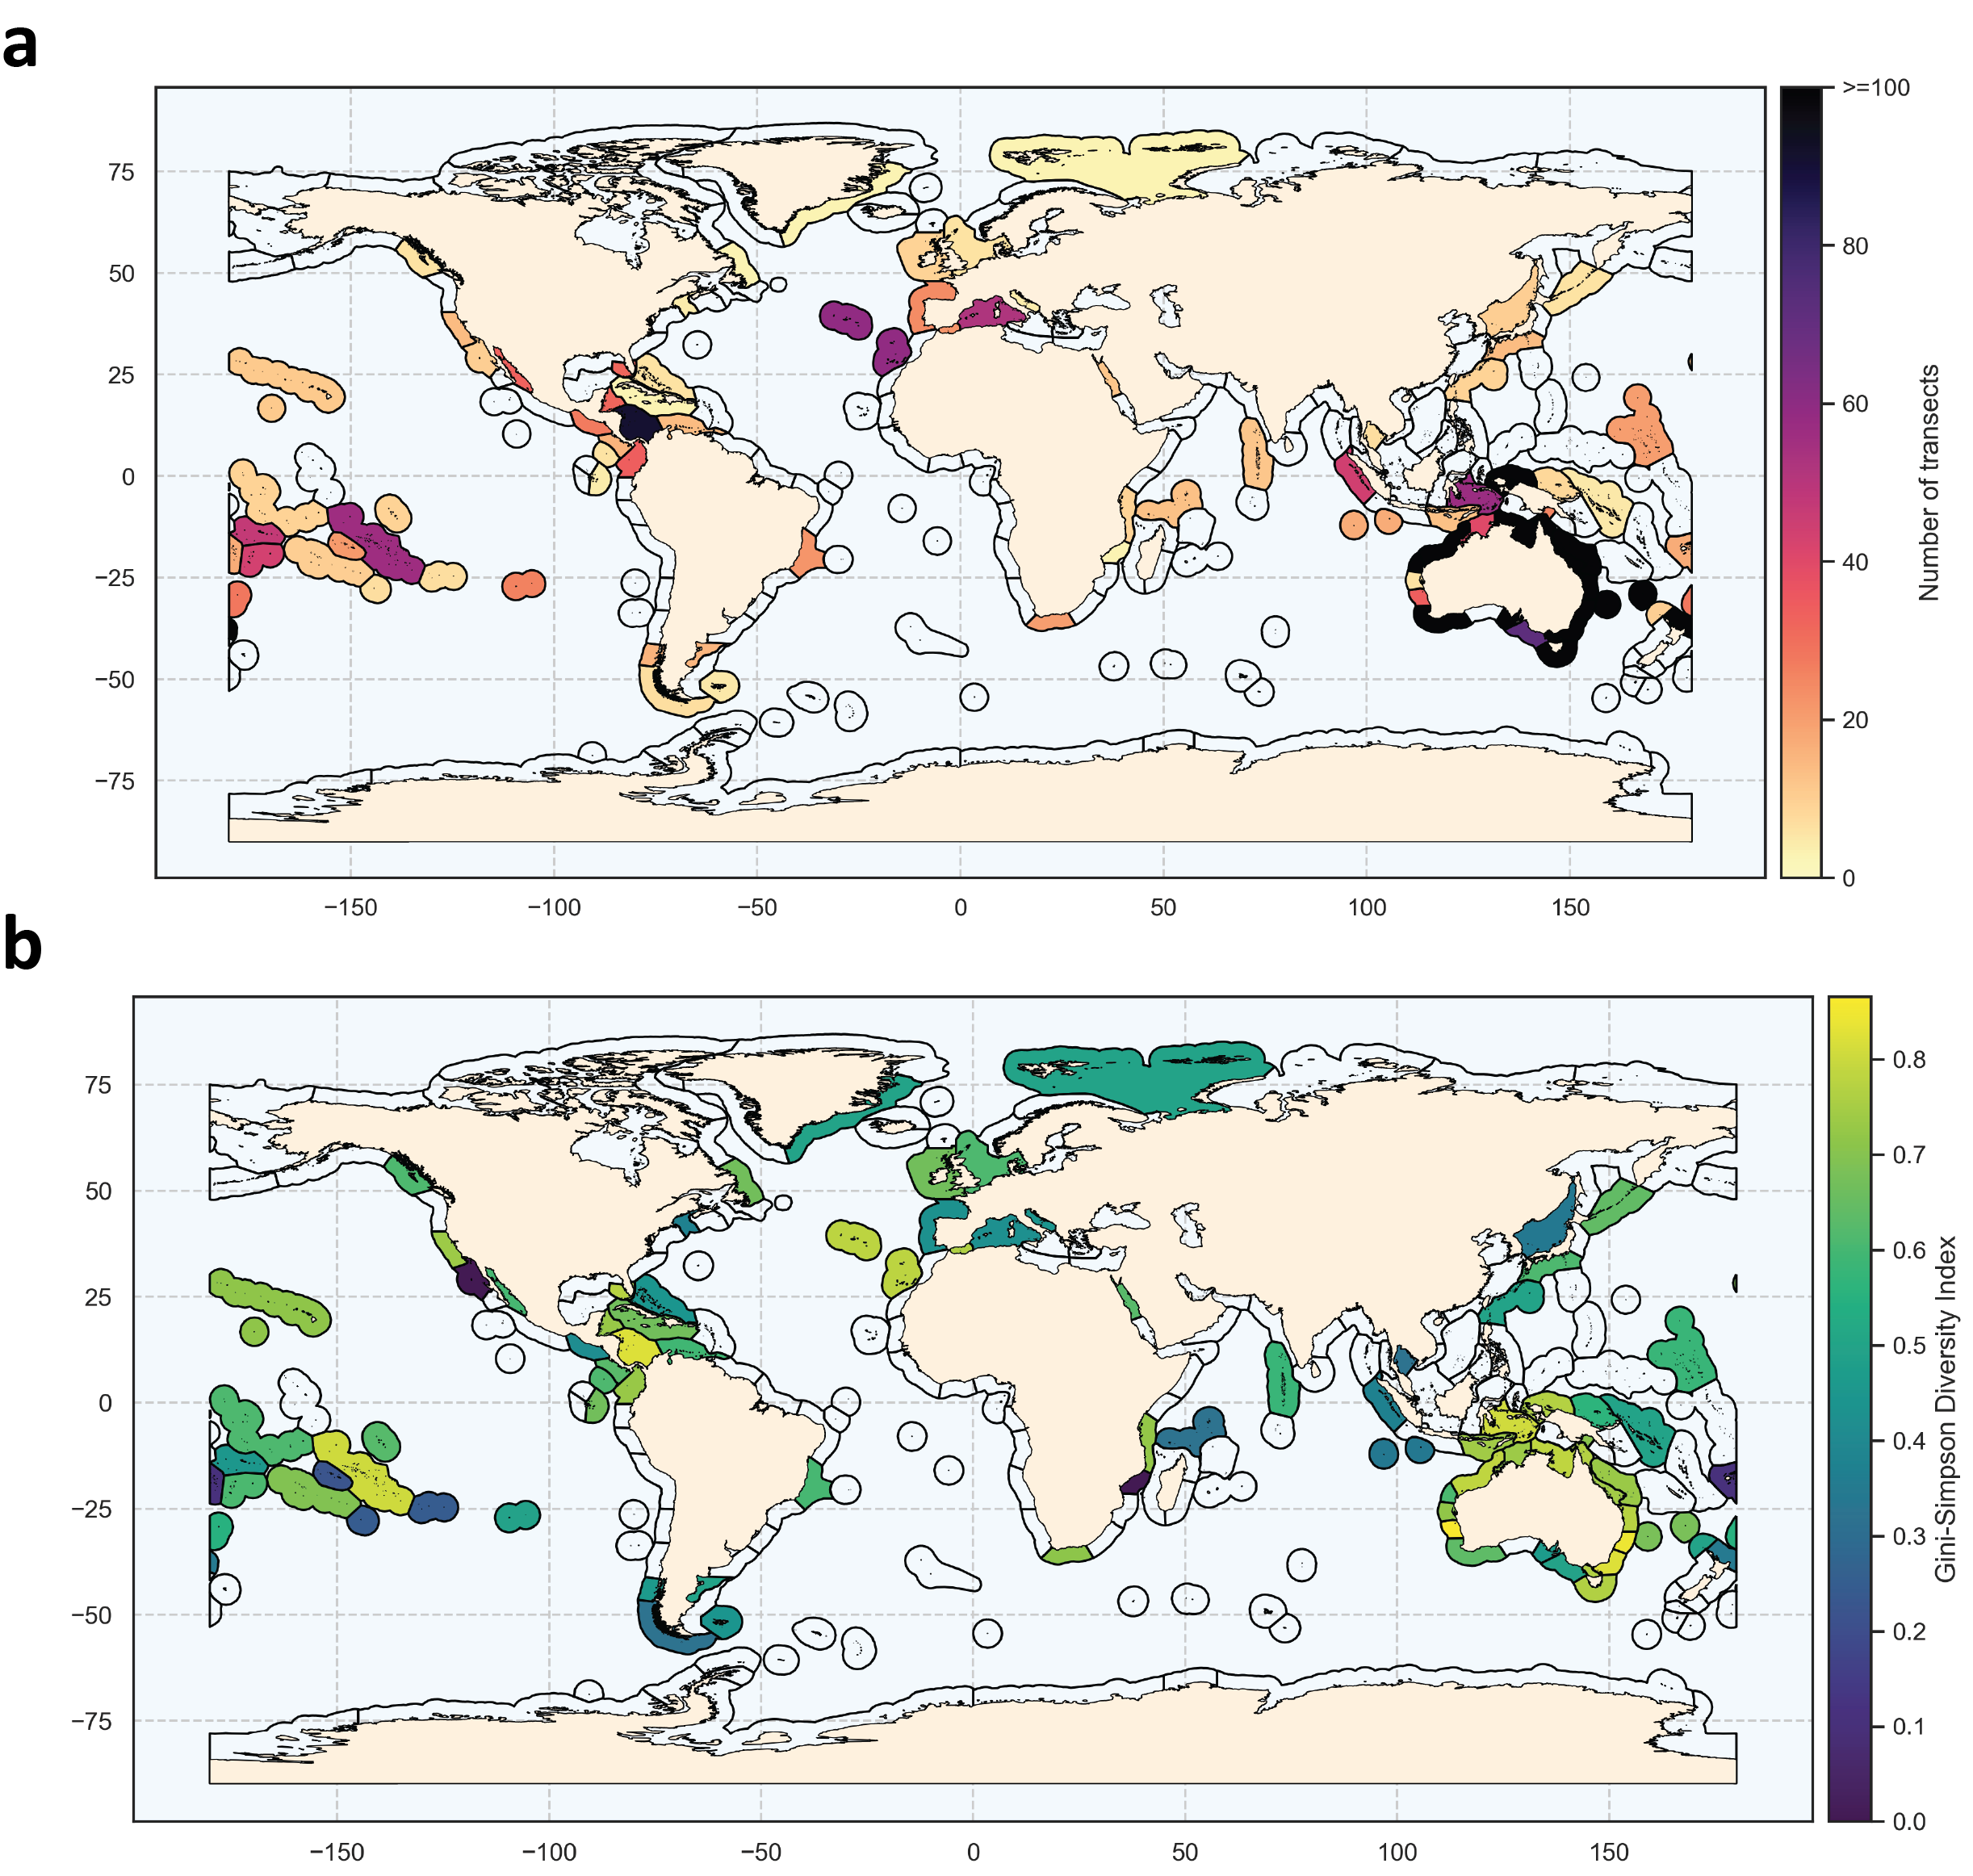
\includegraphics{03-Chapitre2/figures/fig4_ab.png}
\caption{a. Spatial distribution of reef surveys from the Reef Life
Survey database used for analyses. b. Map of dominant clusters in each
MEOW ecoregion. Dominant clusters were determined as the greatest count
of transect labels in each ecoregion. c.~Spatial distribution of the
proportion of transects classified as noise in each ecoregion.
d.~Gini-Simpson diversity index calculated by the occurrence of clusters
in each ecoregion of the world.}\label{fig:chap2fig4}
}
\end{figure}
\begin{figure}
\ContinuedFloat
\centering
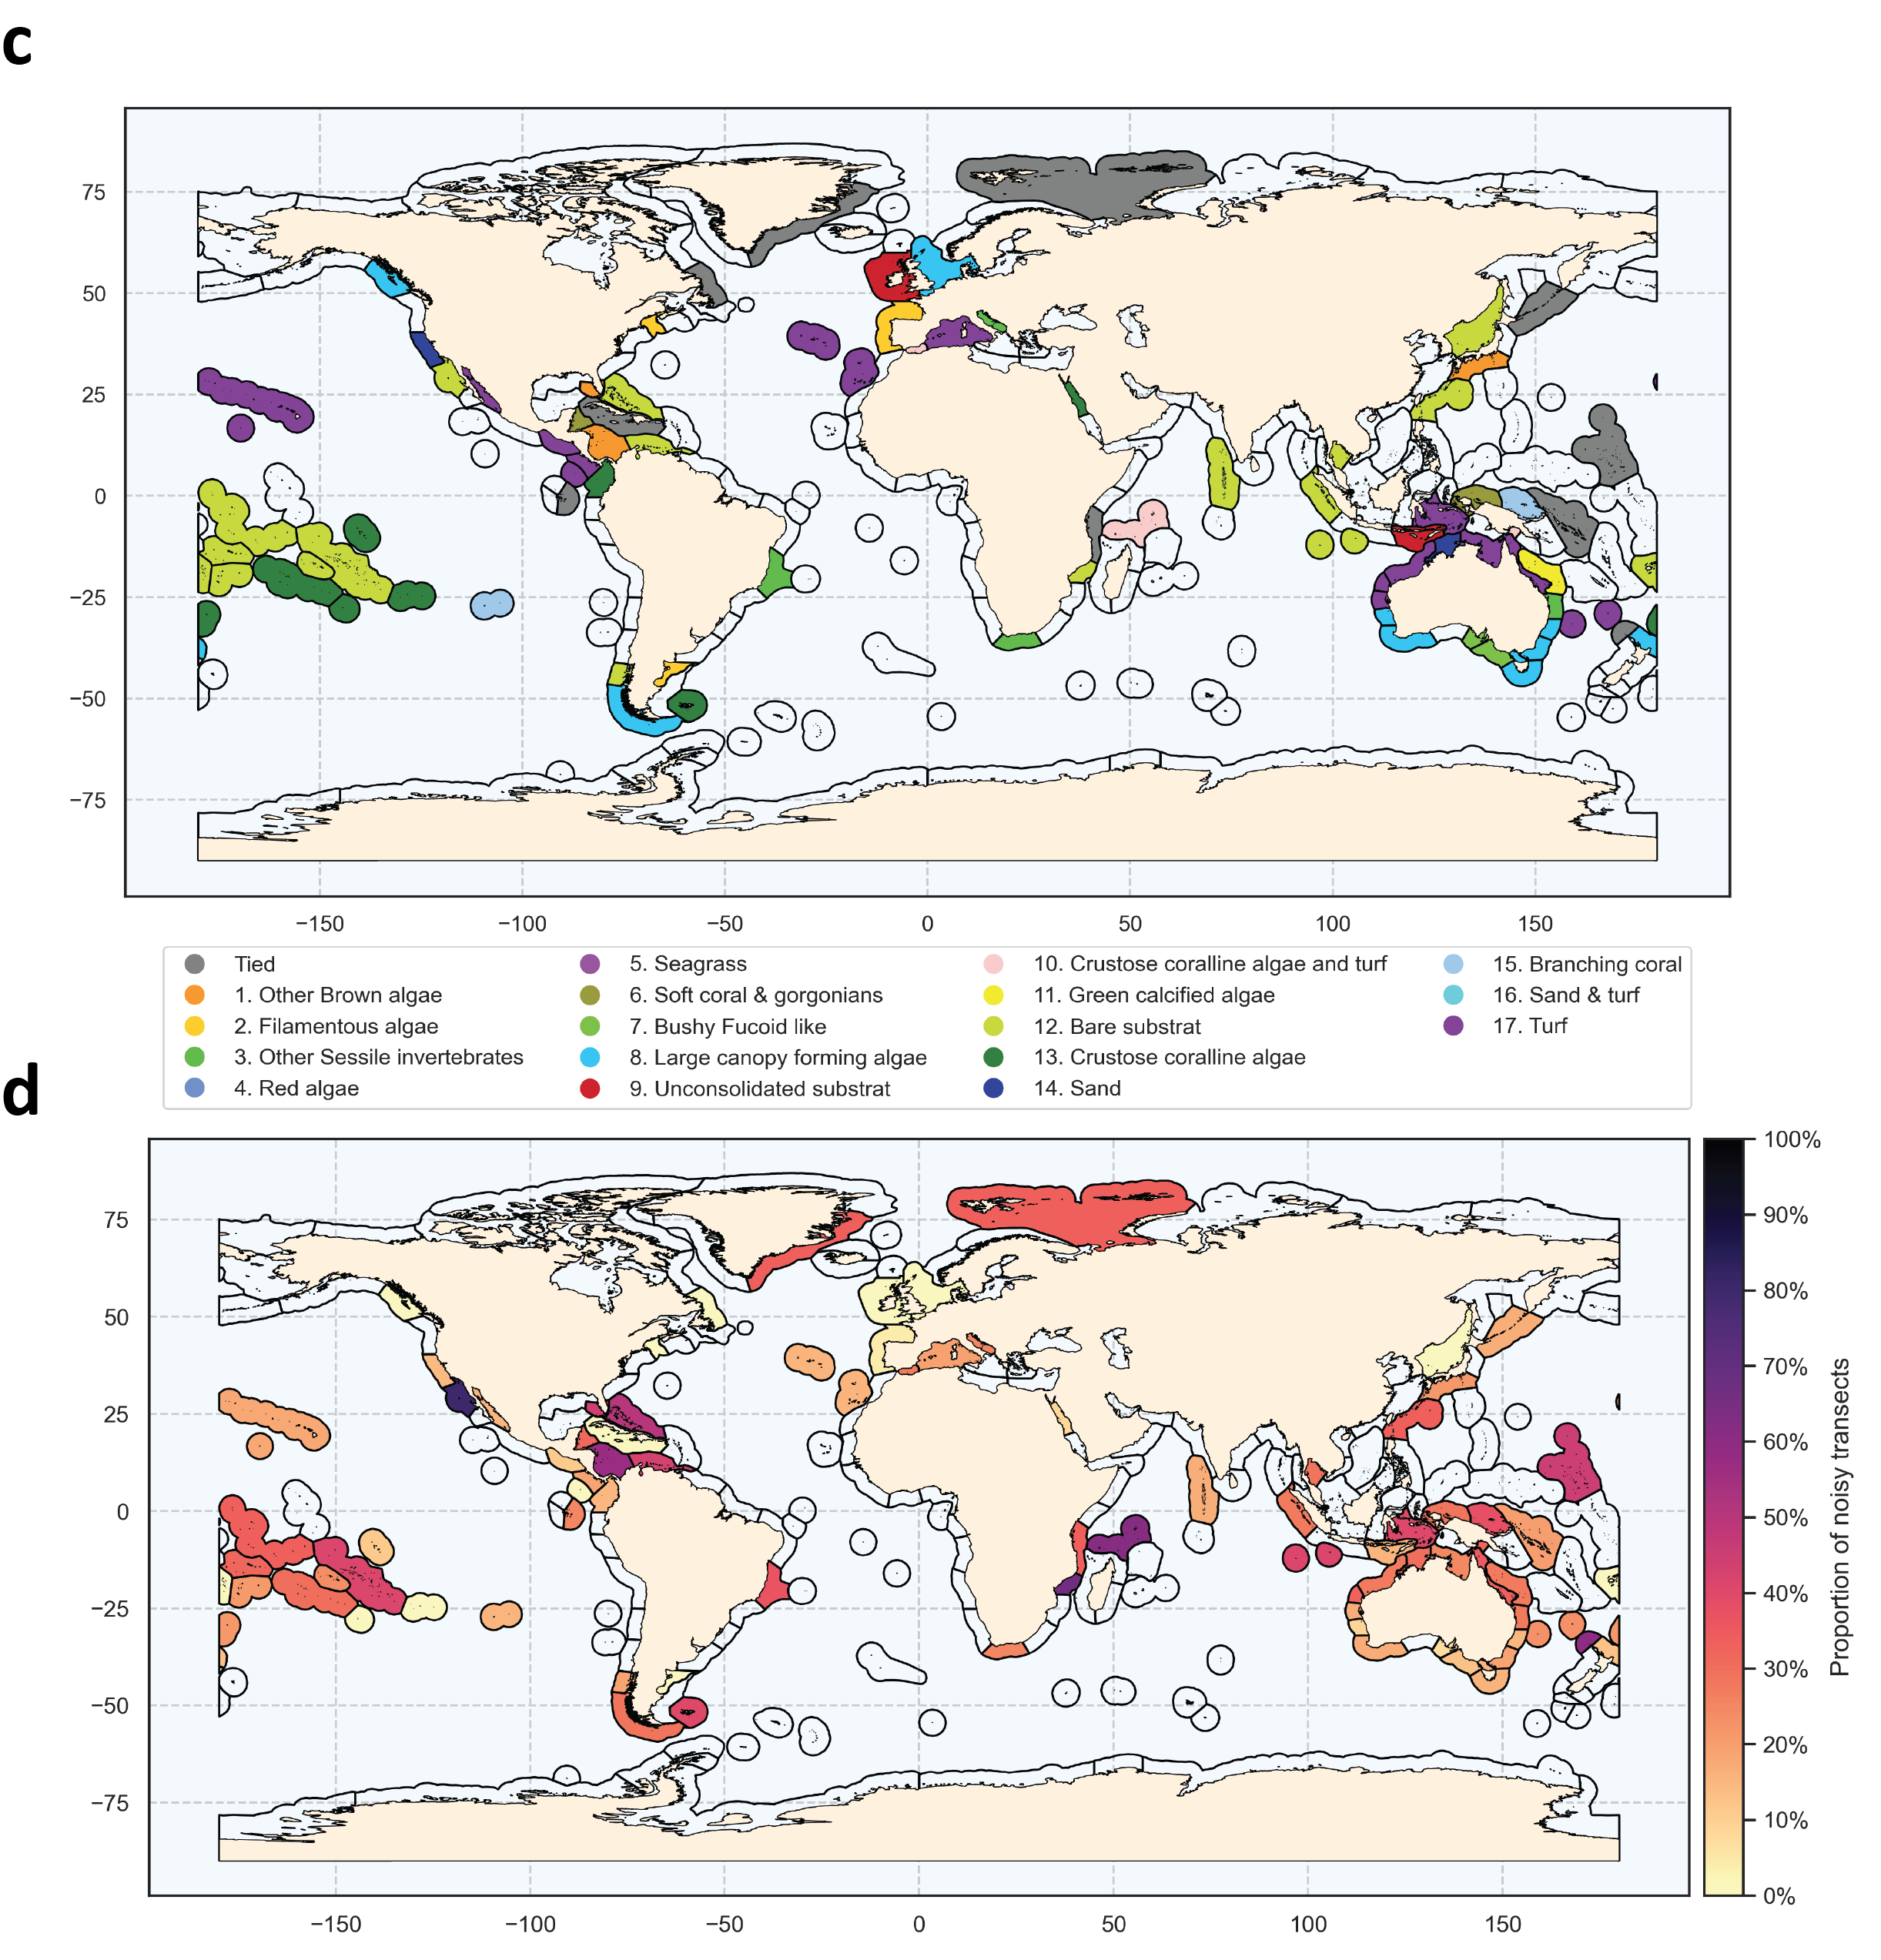
\includegraphics{03-Chapitre2/figures/fig4_cd.png}
\caption[]{a. Spatial distribution of reef surveys from the Reef Life
Survey database used for analyses. b. Map of dominant clusters in each
MEOW ecoregion. Dominant clusters were determined as the greatest count
of transect labels in each ecoregion. c.~Spatial distribution of the
proportion of transects classified as noise in each ecoregion.
d.~Gini-Simpson diversity index calculated by the occurrence of clusters
in each ecoregion of the world.}
\end{figure}

At a finer spatial scale, it is also possible to identify spatial and
temporal transitions in the occurrence of the different clusters
(Fig.~\ref{fig:chap2fig5}). Along spatial gradients, clusters classified
as noise may be a sign of the presence of an ecotone, as in the Cape
Howe region in southeastern Australia (Fig.~\ref{fig:chap2fig5} b).
These transects classified as noise separate an area with transects
classified as bare substrate/crustose coralline algae to the north from
an area to the south with transects classified as canopy forming algae
and red algae (Fig.~\ref{fig:chap2fig5} b).

\begin{figure}
\hypertarget{fig:chap2fig5}{%
\centering
\includegraphics{03-Chapitre2/figures/fig5.png}
\caption[Well-sampled ecoregions in Australia, with high number of
transects and temporal replications between 2008 and 2021.]{Well-sampled ecoregions in Australia, with high number of
transects and temporal replications between 2008 and 2021. b.
Distribution of 44 sites surveyed between 2008 and 2021 in the Cape Howe
region; Colour coding indicates cluster identity. Dots are jittered
along the y-axis. c.~Number and proportion of transects in the different
clusters for the period 2008-2013 in the four ecoregions highlighted in
a. d.~The same analysis for the period 2014-2021.}\label{fig:chap2fig5}
}
\end{figure}

The relative proportion of the different clusters is overall stable
overtime when comparing the early and the late 2010s. In this temperate
zone, the most predominant cluster remains the canopy forming algae,
followed by transects classified as noise (Fig.~\ref{fig:chap2fig5} c).
Noticeable changes between the two periods include: the proportion of
transects classified as sand decreased from 10\% to below 8\%, while the
proportion of transects classified as \emph{turf} increased from 7\% to
exceed 10\% (Fig.~\ref{fig:chap2fig5} c \& d). Transects classified as
\emph{turf} or \emph{crustose coralline and turf} or \emph{sand and
turf}, represented approximately 16\% of the clusters between 2008-2013
and increased to nearly 19\% for the period 2015-2021. The proportion of
transects classified as bare substrate declined from approximately 5\%
in 2008-2013 to only 1\% of the transects in 2015-2021.

\clearpage

\hypertarget{discussion-chapt2}{%
\section{Discussion}\label{discussion-chapt2}}

The \emph{UMAP-HDBSCAN} clustering pipeline identified 17 distinct
clusters within all the \emph{RLS} transects performed globally across a
range of coastal temperate and tropical regions. Within these groups, we
found different biogenic habitats whose distribution patterns match with
current biogeographic knowledge of benthic ecosystems: for example,
\emph{bushy fucoid-like algae}, and \emph{canopy-forming algae}
predominantly occur in temperate waters \autocites[
]{Assis_2020}{Jayathilake_2020}, while \emph{soft corals and
gorgonians}, and \emph{branching coral} are more frequent in tropical
waters \autocites[ ]{Jones_2019}{Wirabuana_2019}. Our analysis also
highlights habitat types that occur across the globe, including (1)
different granulometric facies like \emph{sand}, \emph{unconsolidated
substrate}, and \emph{bare substrate,} as well as (2) different habitat
types dominated by low-profile algae , such as \emph{crustose coralline
algae} or \emph{turf algae}. The latter are known to occur across the
globe and can dominate benthic substrates in diverse conditions
\autocites[ ]{Connell_2014}{Liu_2018}.

In addition, this classification also distinguishes between different
ecological states of these habitats (hereafter refers to as ``habitat
state''), including known alternative successional stages, or different
degradation states of these habitats (Fig.~\ref{fig:chap2fig6}). For
example, the clusters \emph{crustose coralline algae}, \emph{crustose
coralline algae and turf} and \emph{turf} provide an interesting
template to describe the habitat transitions described in
\textcite{Cornwall_2023}, which suggests that a shift from
\emph{crustose coralline algae} to \emph{turf} domination reduces reef
carbonate production. Similarly, the clusters \emph{branching coral},
\emph{turf and sand} and \emph{turf} can be used to describe and
quantify in a standardised manner the transitions between corals and
turf dominated habitats that are occurring more frequently due to
anthropogenic pressures \autocite{Jouffray_2015}.
Fig.~\ref{fig:chap2fig5} b also illustrates the occurrence along the
southeastern Australian coastline of alternative ecological states on
temperate reefs, where dense macroalgal canopies dominated by
\emph{Ecklonia radiata} (here \emph{large canopy-forming algae}), can
shift to extensive barrens (here \emph{bare substrate} or \emph{crustose
coralline algae}) following destructive grazing by the long-spined sea
urchin \emph{Centrostephanus rodgersii} \autocite{Ling_2009}. Thus, our
approach can classify reef cover data collected across the globe with
the \emph{RLS} protocol into an ecologically sound template to explore
common reef habitat transitions under anthropogenic pressures
\autocite{Donovan_2018}.

\begin{figure}
\hypertarget{fig:chap2fig6}{%
\centering
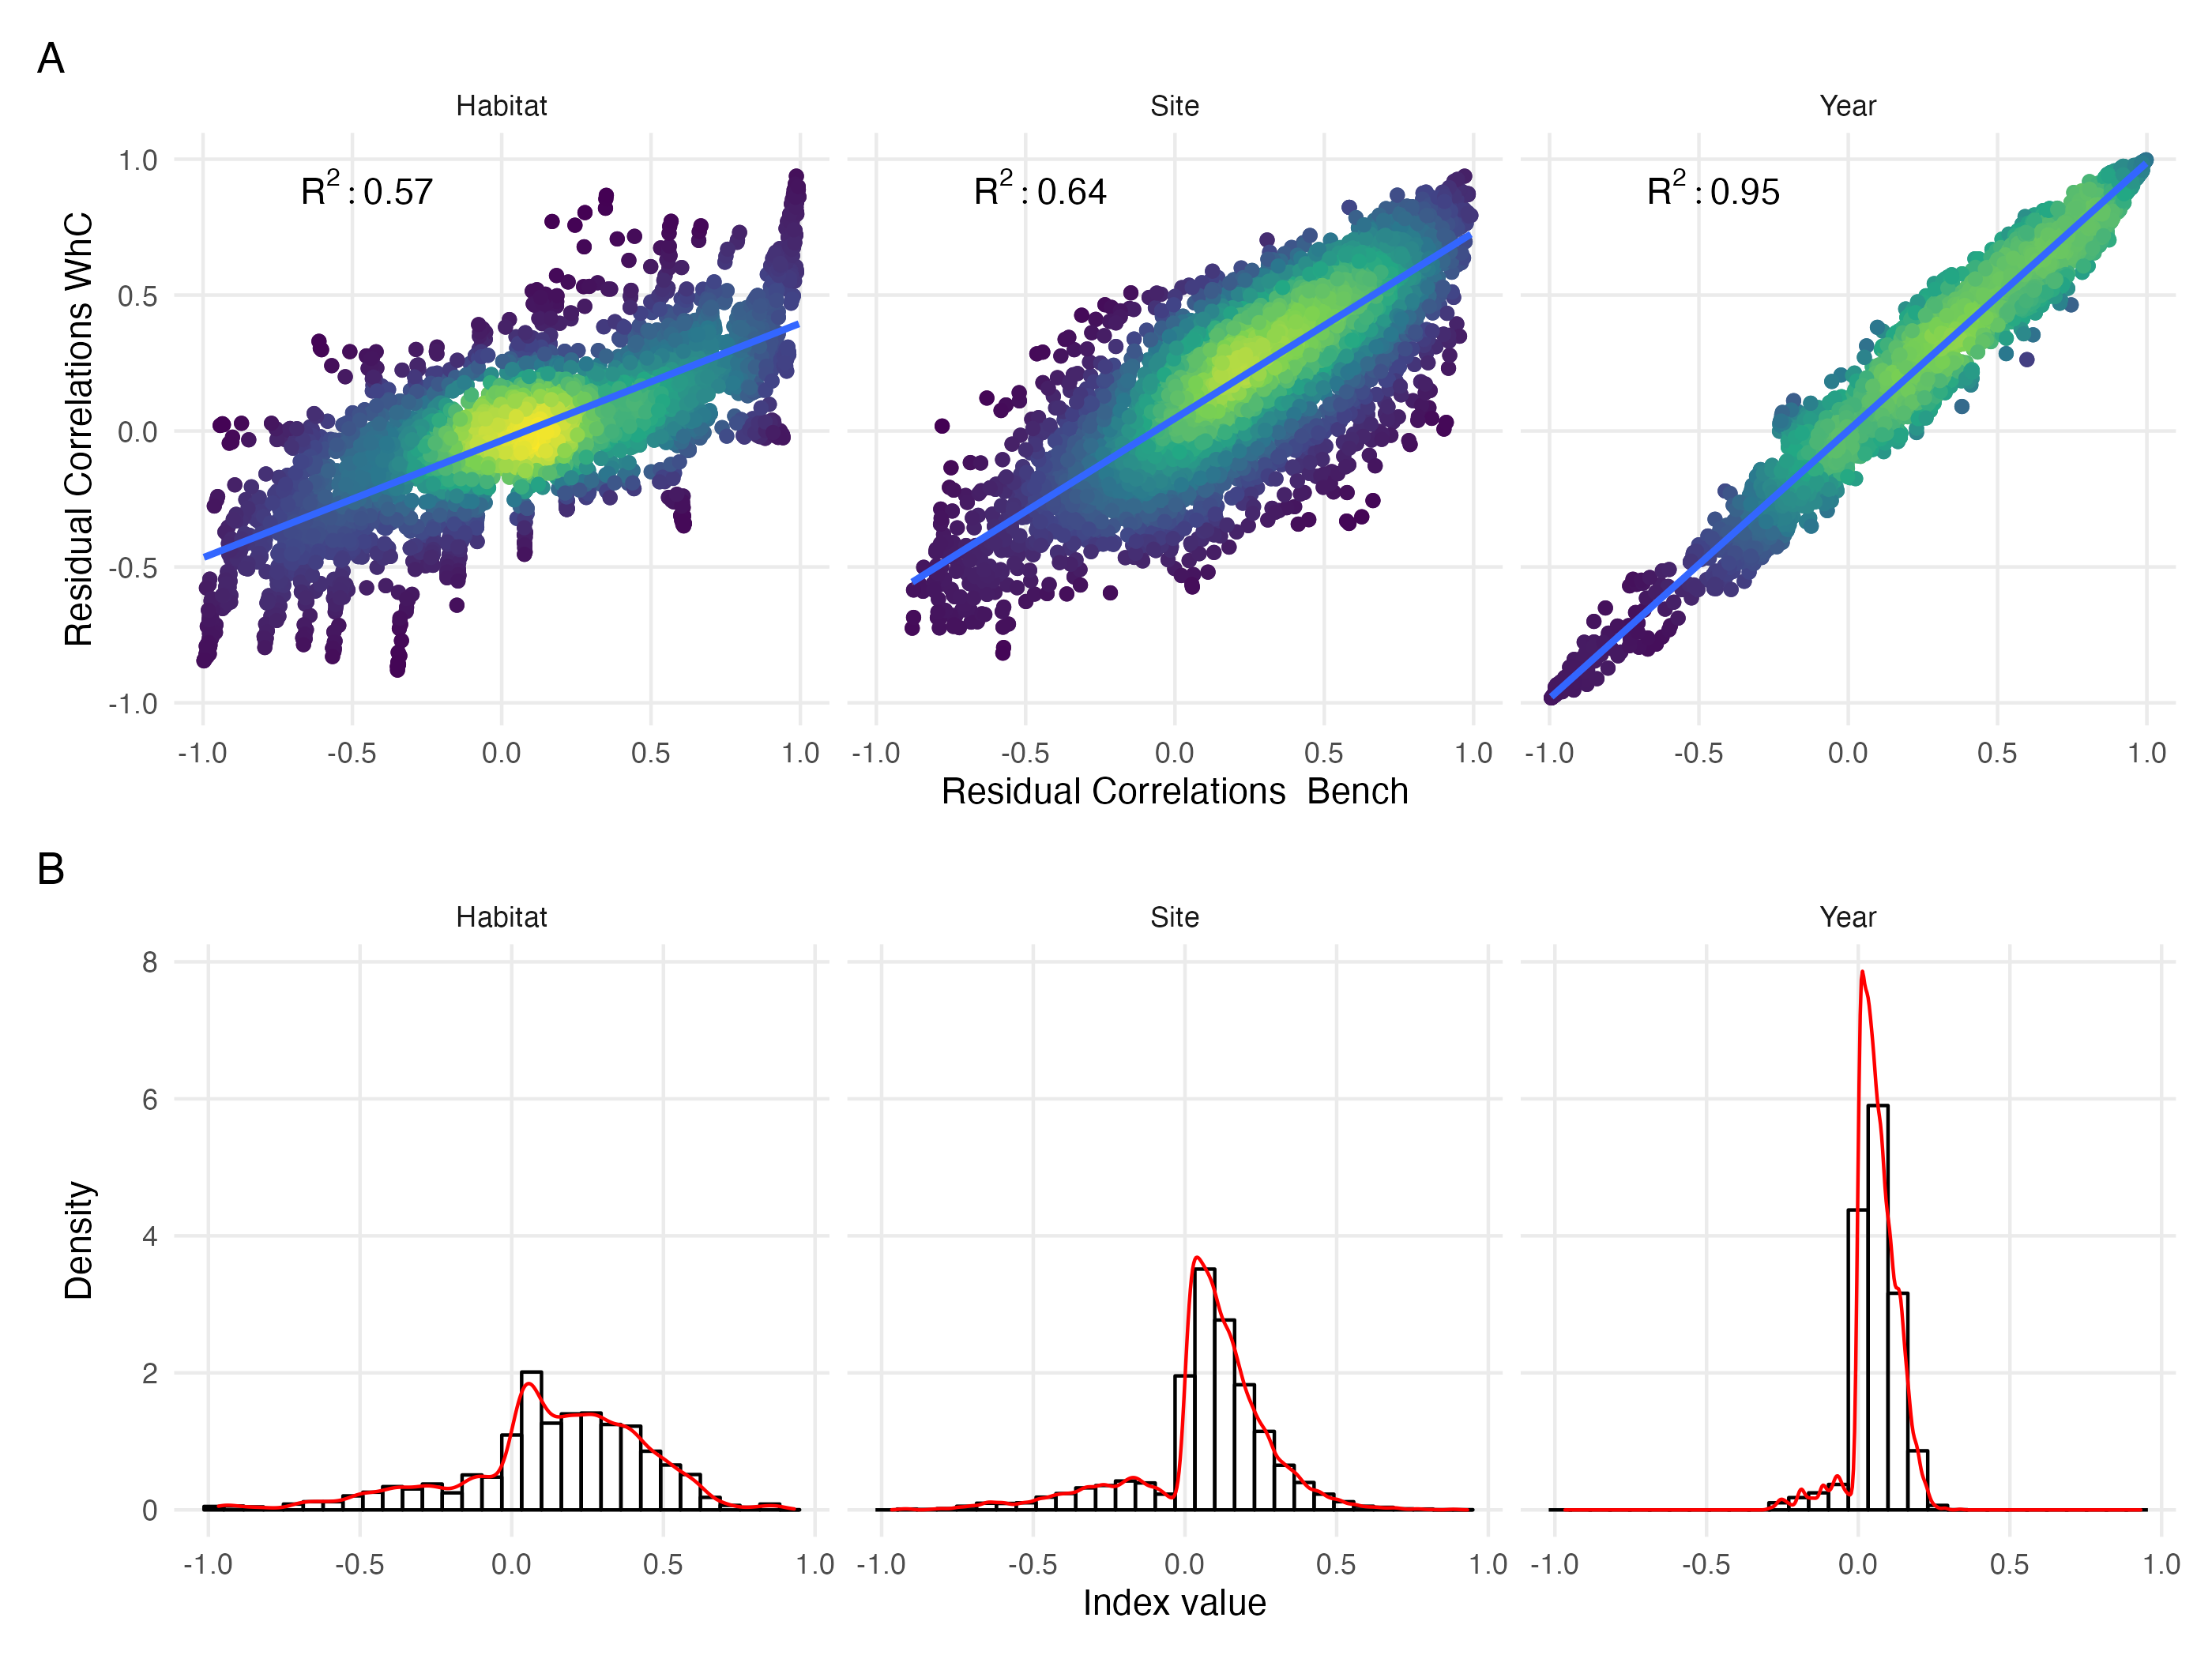
\includegraphics{03-Chapitre2/figures/fig6.png}
\caption[Two-dimensional UMAP embedding of the 5,090 clustered
\emph{RLS} transects.]{Two-dimensional UMAP embedding of the 5,090 clustered
\emph{RLS} transects. Each picture is representative of its cluster. The
arrows indicate potential transitions as identified in
\textcite{Jouffray_2015} and
\textcite{Cornwall_2023}.}\label{fig:chap2fig6}
}
\end{figure}

Certain of the habitat states identified here on the global \emph{RLS}
dataset match well with the habitat states previously identified by
\textcite{Cresswell_2017}, who applied another clustering approach to an
Australian subset of the \emph{RLS} dataset. In particular, some of our
groups (i.e.~\emph{canopy forming algae}, \emph{turf algae},
\emph{filamentous algae} and \emph{branching coral}), match well with
four out of the nine habitat states identified by
\textcite{Cresswell_2017} (i.e.~''Canopy algae'', ``Turf'', ``Epiphytic
filamentous algae--caulerpa'' and ``Coral''; see Table 1 in
\textcite{Cresswell_2017} for a detailed description of their habitat
states and Fig.~\ref{fig:chap2fig2} b in this paper for comparison).
Furthermore, we identified more finely-resolved habitat states here
relative to the classification proposed by \textcite{Cresswell_2017}.
The clusters \emph{crustose coralline algae} and \emph{bare substrate}
identified here are amalgamated into a single ``Barren'' cluster in
\textcite{Cresswell_2017}, while the clusters \emph{red algae} and
\emph{other brown algae} further detail what \textcite{Cresswell_2017}
identified as one single ``Foliose algae'' group. Thus, our large-scale
spatial approach overall confirms the habitat types defined by
\textcite{Cresswell_2017} while to some extent providing a more nuanced
distinction between similar habitats. Nevertheless, our analysis only
managed to capture one type of coral reef, contrary to what we might
have expected, but there may be several reasons for this result. The
proportion of coral cover within coral reefs exhibits significant
variability, as indicated by \autocite{Death_2012}, although multiple
sub-categories of coral have been merged together to circumvent this
issue (see Appendix A Table S1). Additionally, the morphological
diversity of these reefs is extensive, with variations in surface areas
\autocite{Zawada_2019}. Such variability might elucidate why a singular
group of corals, \emph{Branching coral} is found as a group, since some
species of \emph{Acropora spp.} are able to establish colonies with
expansive surface areas. Hence, our data-driven approach yields a finely
resolved classification that comprises typical benthic habitats
(e.g.~seagrass meadows, coral reefs, kelp forests) that are common
across all major seafloor habitat classification scheme
(e.g.~\emph{European Nature Information System};
\textcite{Bajjouk_2015}).

Our global classification of the \emph{RLS} data highlights hotspots of
diversity in terms of benthic habitats and habitat states. Four
ecoregions in particular, the Eastern (Manning-Hawkesbury ecoregion) and
Western Australia (Houtman ecoregion), the Caribbean, and the Tuamotus
Archipelago, showed a high diversity of habitat types (considering both
richness and evenness). The high diversity of habitat types we report in
the Caribbean and in the Tuamotus Archipelago potentially contribute to
explain the high marine diversity of reef fishes reported in these
tropical coral reefs, despite their small area at a global scale
\autocite{Cowman_2017}. In the transition zones between temperate and
tropical waters, such as the Manning-Hawkesbury or the Houtman
ecoregions in eastern and western Australia respectively, the high
diversity of benthic habitat types we observe could be explained by a
high diversity of foundation species. Indeed, high biodiversity is
typical of transitional environmental conditions where ecological
niches, which are overall disjointed, overlap \autocite{Ferro_2014}.
This phenomenon is well known for multiple taxon such as birds
\autocite{Altamirano_2020}, plants \autocite{Lemessa_2023} or reef fish
\autocite{Pinheiro_2018} and also seems to apply to a certain extent to
biogenic habitats like coralline red algae \autocite{Sissini_2022}. Such
subtropical or warm temperate zones are also identified as regions where
both mobile fauna \autocite{Verges_2014} or sessile habitat-forming
species assemblages \autocite{Marzloff_2018} are likely to undergo
tropicalisation, which implies that native temperate assemblages can
co-occur with warmer species assemblages undergoing poleward
climate-driven range shifts. Our finely resolved classification could be
modelled against environmental predictors in future work to understand
and predict the state of benthic habitats under current and future
conditions (e.g. \textcite{Belanger_2012}).

Beyond exploring spatial patterns of benthic biodiversity, our
classification of the \emph{RLS} dataset offers a new perspective to
explore temporal changes in benthic habitat states. Within the most
resampled ecoregions (essentially located in southeastern Australia), we
quantified temporal changes in the occurrence of certain habitat types
between the period 2008-2013 and 2014-2021. For example, the proportion
of transects classified as \emph{large canopy-forming algae} shows an
increase in the Manning-Hawkesbury ecoregion (Fig. S39 in Supplementary
Informations) while it decreased in the Cape Howe ecoregion (Fig. S40 in
Supplementary Informations). These regional differences can be explained
by local changes in the environment \autocite{Krumhansl_2016}. We also
observe an increase in transects classified as \emph{turf algae} among
the five ressampled ecoregions (e.g.~+67\% increase between the two
periods), in line with findings of an increase in turf algae due to both
global climate change and local anthropogenic impacts
\autocite{Filbee-Dexter_2018}. Note, however, that temporal analysis of
changes was restricted to only 5 southeastern Australian data-rich
ecoregions out of a total of 232 worldwide. This reflects the strong
geographical bias of the \emph{RLS} dataset, with 78\% of transects
performed along Australian shores. Moreover, marginal changes in the
proportion of certain habitat states, such as \emph{red algae} or
\emph{seagrass}, may also be due to the random positioning of transects,
which does make the survey protocol accessible to citizen scientists but
does not guarantee truly replicated observations through time.

Beyond exploring spatial patterns of benthic biodiversity, our
classification of the \emph{RLS} dataset offers a new perspective to
explore temporal changes in benthic habitat states. Within the most
frequently sampled ecoregions (essentially located in southeastern
Australia), we quantified temporal changes in the occurrence of certain
habitat types between the period 2008-2013 and 2014-2021. The proportion
of transects classified as \emph{large canopy-forming algae} shows an
increase in the Manning-Hawkesbury ecoregion (Fig. S39 in Supplementary
Informations) while it decreased in the Cape Howe ecoregion (Fig. S40 in
Supplementary Informations). These regional differences can be explained
by local changes in the environment \autocite{Krumhansl_2016}, including
poleward expansion of urchin barrens \autocite{Ling_2018}. We also
observe an increase in transects classified as \emph{turf algae} among
the five ressampled ecoregions (e.g.~+67\% increase between the two
periods), in line with findings of an increase in \emph{turf algae} due
to both global climate change and local anthropogenic impacts
\autocite{Filbee-Dexter_2018}. Note, however, that temporal analysis of
changes was restricted to only 5 southeastern Australian data-rich
ecoregions out of a total of 232 worldwide. This was due to the
distribution of data availability, which is heavily focussed within the
region that \emph{RLS} originated from (southern Australia). Moreover,
marginal changes in the proportion of certain habitat states, such as
\emph{red algae} or \emph{seagrass}, may also be due to the random
positioning of transects within a site through time (as opposed to
fixed). This is beneficial for greater site replication and for
application by citizen scientists, but adds an extra source of noise to
observations within sites through time.

Overall benthic habitat changes may reflect a range of processes,
including ecological ones such as temporal variability in the cover of
habitat-forming species (e.g. \textcite{Wernberg_2016}) in relation to
climate-driven environmental changes (i.e.~tropicalisation of
tropical-temperate transition zones \autocite{Horta_2014}, marine
heatwaves \autocite{Wernberg_2016}) or to trends in human stressors (i.e
nutrients and organic pollution runoffs, impacts from coastal human
populations; \textcite{Halpern_2019}), as well as methodological ones,
such as variability in transect location or in sampling effort through
time (e.g. \textcite{Stuble_2021}). Identifying the processes driving
the observed habitat transitions could help better characterise the
impact of anthropogenic activities on benthic habitats (see for example
\textcite{Donovan_2018} for a similar approach at a finer spatial
scale). Our classification could thus provide an interesting template to
further explore changes in benthic habitats across the world
\autocite{Edgar_2023}.

Nonetheless, not all expected transitions between habitats, or
alternative ecological states, come out in the different clusters. Some
transitory states may be classified as noise if they are too scarcely
observed in the dataset to constitute a cluster of their own.
Understanding the drivers behind the transects classified as noise can
reveal valuable information about the factors influencing habitat
variability and the ecological processes driving shifts between
different states. This includes deciphering the reasons for a noise
classification, such as variations in environmental conditions, biotic
interactions, or anthropogenic disturbances. By investigating these
aspects, researchers can gain crucial insights into the dynamics and
transitions occurring between habitat states and alternative ecological
states.

The \emph{UMAP-HDBSCAN} clustering pipeline presented in this study
demonstrates remarkable robustness and versatility, leveraging global
data to identify fine-scale patterns within coastal temperate and
tropical ecosystems. Because of its hierarchical structure, this
pipeline aligns well with established classification standards and
facilitates a first data-driven description of global patterns in
habitat states, which constitutes a valuable database to explore the
influence of local and global drivers of benthic habitat states.
Additionally, the pipeline's capability to handle non-linear data and
accommodate noise underscores its adaptability to various ecological
contexts and data sources (e.g.~citizen science).

\clearpage

\printbibliography[heading=subbibintoc, title={Bibliographie}]
\end{refsection}
\clearpage
\printbibliography[heading=subbibintoc, title={Bibliographie}]
\clearemptydoublepage

\hypertarget{nom-du-chapitre-3}{%
\chapter{Nom du chapitre 3}\label{nom-du-chapitre-3}}

Lorem ipsum dolor sit amet, «\textsubscript{consectetuer}» adipiscing
elit. Maecenas fermentum, elit non lobortis cursus, orci velit suscipit
est, id mollis turpis mi eget orci. Ut aliquam sollicitudin metus.
Mauris at sapien sed sapien congue iaculis. Nulla lorem urna, bibendum
id, laoreet iaculis, nonummy eget, massa. Phasellus ullamcorper commodo
velit. Class aptent taciti sociosqu ad litora torquent per
«\textasciitilde conubia nostra\textasciitilde», per inceptos hymenaeos.
Phasellus est. Maecenas felis augue, gravida quis, porta adipiscing,
iaculis vitae, felis. Nullam ipsum. Nulla a sem ac leo fringilla mattis.
Phasellus egestas augue in sem. Etiam ac enim non mauris ullamcorper
scelerisque. In wisi leo, malesuada vulputate, tempor sit amet,
facilisis vel, velit. Mauris massa est, sodales placerat, luctus id,
hendrerit a, urna. Nullam eleifend pede eget odio. Duis non erat. Nullam
pellentesque \autocite{Doule1887}.

\hypertarget{premiuxe8re-section-du-chapitre}{%
\section{Première section du
chapitre}\label{premiuxe8re-section-du-chapitre}}

\hypertarget{premiuxe8re-sous-section}{%
\subsection{Première sous-section}\label{premiuxe8re-sous-section}}

Cras molestie. Curabitur id urna. Suspendisse tempor. Aliquam erat
volutpat. Aliquam erat volutpat. Nam ultricies metus sit amet
erat\footnote{Mauris neque odio, ornare id, rhoncus non, sollicitudin sed, lectus. Phasellus et dolor. Aenean ullamcorper risus id libero. Pellentesque ac sem eget libero aliquam tincidunt. Suspendisse neque.}.
Suspendisse eget ipsum ut purus imperdiet suscipit. Mauris sed urna at
diam volutpat placerat. Nulla vitae tortor. Nulla sed nisl.

Morbi lorem. Etiam scelerisque rhoncus orci. Nunc elementum ante ac leo.
Vestibulum venenatis dictum nunc. Donec turpis est, dictum nec
\autocite{Drocher2006}, fringilla nec, cursus id, quam. In nibh orci,
porttitor ut, rutrum id, faucibus vitae, leo. Donec ut wisi. Vivamus
ornare, lorem quis tristique dapibus, nulla nisl nonummy libero, vitae
luctus sem felis vel nisl. Suspendisse lectus lacus, ultricies vitae,
feugiat et, hendrerit in, quam. Pellentesque porttitor enim at lectus.
Praesent viverra laoreet velit. Mauris neque odio, ornare id, rhoncus
non, sollicitudin sed, lectus. Phasellus et dolor. Aenean ullamcorper
risus id libero. Pellentesque ac sem eget libero aliquam tincidunt.
Suspendisse neque. Curabitur egestas neque ultrices nisl. Nulla bibendum
augue et tellus. Duis ultrices convallis est.

Lorem ipsum dolor sit amet, consectetuer adipiscing elit. Maecenas
fermentum, elit non lobortis cursus, orci velit suscipit est, id mollis
turpis mi eget orci. Ut aliquam sollicitudin metus. Mauris at sapien sed
sapien congue iaculis. Nulla lorem urna, bibendum id, laoreet iaculis,
nonummy eget, massa. Phasellus ullamcorper commodo velit. Class aptent
taciti sociosqu ad litora torquent per conubia nostra, per inceptos
hymenaeos. Phasellus est. Maecenas felis augue, gravida quis, porta
adipiscing, iaculis vitae, felis. Nullam ipsum. Nulla a sem ac leo
fringilla mattis. Phasellus egestas augue in sem. Etiam ac enim non
mauris ullamcorper scelerisque. In wisi leo, malesuada vulputate, tempor
sit amet, facilisis vel, velit. Mauris massa est, sodales placerat,
luctus id, hendrerit a, urna. Nullam eleifend pede eget odio. Duis non
erat. Nullam pellentesque.

\hypertarget{deuxiuxe8me-sous-section}{%
\subsection{Deuxième sous-section}\label{deuxiuxe8me-sous-section}}

Morbi lorem. Etiam scelerisque rhoncus orci. Nunc elementum ante ac leo.
Vestibulum venenatis dictum nunc. Donec turpis est, dictum nec,
fringilla nec, cursus id, quam. In nibh orci, porttitor ut, rutrum id,
faucibus vitae, leo. Donec ut wisi. Vivamus ornare, lorem quis tristique
dapibus, nulla nisl nonummy libero, vitae luctus sem felis vel nisl.
Suspendisse lectus lacus, ultricies vitae, feugiat et, hendrerit in,
quam. Pellentesque porttitor enim at lectus. Praesent viverra laoreet
velit. Mauris neque odio, ornare id, rhoncus non, sollicitudin sed,
lectus. Phasellus et dolor. Aenean ullamcorper risus id libero.
Pellentesque ac sem eget libero aliquam tincidunt. Suspendisse neque.
Curabitur egestas neque ultrices nisl. Nulla bibendum augue et tellus.
Duis ultrices convallis est.

Lorem ipsum dolor sit amet, consectetuer adipiscing elit. Maecenas
fermentum, elit non lobortis cursus, orci velit suscipit est, id mollis
turpis mi eget orci. Ut aliquam sollicitudin metus. Mauris at sapien sed
sapien congue iaculis. Nulla lorem urna, bibendum id, laoreet iaculis,
nonummy eget, massa. Phasellus ullamcorper commodo velit. Class aptent
taciti sociosqu ad litora torquent per conubia nostra, per inceptos
hymenaeos. Phasellus est. Maecenas felis augue, gravida quis, porta
adipiscing, iaculis vitae, felis. Nullam ipsum. Nulla a sem ac leo
fringilla mattis. Phasellus egestas augue in sem. Etiam ac enim non
mauris ullamcorper scelerisque. In wisi leo, malesuada vulputate, tempor
sit amet, facilisis vel, velit. Mauris massa est, sodales placerat,
luctus id, hendrerit a, urna. Nullam eleifend pede eget odio. Duis non
erat. Nullam pellentesque.

Lorem ipsum dolor sit amet, consectetuer adipiscing elit. Maecenas
fermentum, elit non lobortis cursus, orci velit suscipit est, id mollis
turpis mi eget orci. Ut aliquam sollicitudin metus. Mauris at sapien sed
sapien congue iaculis. Nulla lorem urna, bibendum id, laoreet iaculis,
nonummy eget, massa. Phasellus ullamcorper commodo velit. Class aptent
taciti sociosqu ad litora torquent per conubia nostra, per inceptos
hymenaeos. Phasellus est. Maecenas felis augue, gravida quis, porta
adipiscing, iaculis vitae, felis. Nullam ipsum. Nulla a sem ac leo
fringilla mattis. Phasellus egestas augue in sem. Etiam ac enim non
mauris ullamcorper scelerisque. In wisi leo, malesuada vulputate, tempor
sit amet, facilisis vel, velit. Mauris massa est, sodales placerat,
luctus id, hendrerit a, urna. Nullam eleifend pede eget odio. Duis non
erat. Nullam pellentesque.

\hypertarget{conclusion-du-troisiuxe8me-chapitre}{%
\section{Conclusion du troisième
chapitre}\label{conclusion-du-troisiuxe8me-chapitre}}

Lorem ipsum dolor sit amet, consectetuer adipiscing elit. Maecenas
fermentum, elit non lobortis cursus, orci velit suscipit est, id mollis
turpis mi eget orci. Ut aliquam sollicitudin metus. Mauris at sapien sed
sapien congue iaculis. Nulla lorem urna, bibendum id, laoreet iaculis,
nonummy eget, massa. Phasellus ullamcorper commodo velit. Class aptent
taciti sociosqu ad litora torquent per conubia nostra, per inceptos
hymenaeos. Phasellus est. Maecenas felis augue, gravida quis, porta
adipiscing, iaculis vitae, felis. Nullam ipsum. Nulla a sem ac leo
fringilla mattis. Phasellus egestas augue in sem. Etiam ac enim non
mauris ullamcorper scelerisque. In wisi leo, malesuada vulputate, tempor
sit amet, facilisis vel, velit. Mauris massa est, sodales placerat,
luctus id, hendrerit a, urna. Nullam eleifend pede eget odio. Duis non
erat. Nullam pellentesque.

Lorem ipsum dolor sit amet, consectetuer adipiscing elit. Maecenas
fermentum, elit non lobortis cursus, orci velit suscipit est, id mollis
turpis mi eget orci. Ut aliquam sollicitudin metus. Mauris at sapien sed
sapien congue iaculis. Nulla lorem urna, bibendum id, laoreet iaculis,
nonummy eget, massa. Phasellus ullamcorper commodo velit. Class aptent
taciti sociosqu ad litora torquent per conubia nostra, per inceptos
hymenaeos. Phasellus est. Maecenas felis augue, gravida quis, porta
adipiscing, iaculis vitae, felis. Nullam ipsum. Nulla a sem ac leo
fringilla mattis. Phasellus egestas augue in sem. Etiam ac enim non
mauris ullamcorper scelerisque. In wisi leo, malesuada vulputate, tempor
sit amet, facilisis vel, velit. Mauris massa est, sodales placerat,
luctus id, hendrerit a, urna. Nullam eleifend pede eget odio. Duis non
erat. Nullam pellentesque.

\clearpage
\printbibliography[heading=subbibintoc, title={Bibliographie}]
\clearemptydoublepage

\hypertarget{conclusion}{%
\chapter*{Conclusion}\label{conclusion}}
\addcontentsline{toc}{chapter}{Conclusion}

Lorem ipsum dolor sit amet, «\textsubscript{consectetuer}» adipiscing
elit. Maecenas fermentum, elit non lobortis cursus, orci velit suscipit
est, id mollis turpis mi eget orci. Ut aliquam sollicitudin metus.
Mauris at sapien sed sapien congue iaculis. Nulla lorem urna, bibendum
id, laoreet iaculis, nonummy eget, massa. Phasellus ullamcorper commodo
velit. Class aptent taciti sociosqu ad litora torquent per
«\textasciitilde conubia nostra\textasciitilde», per inceptos hymenaeos.
Phasellus est. Maecenas felis augue, gravida quis, porta adipiscing,
iaculis vitae, felis. Nullam ipsum. Nulla a sem ac leo fringilla mattis.
Phasellus egestas augue in sem. Etiam ac enim non mauris ullamcorper
scelerisque. In wisi leo, malesuada vulputate, tempor sit amet,
facilisis vel, velit. Mauris massa est, sodales placerat, luctus id,
hendrerit a, urna. Nullam eleifend pede eget odio. Duis non erat. Nullam
pellentesque.

Maître Corbeau, sur un arbre perché, Tenait en son bec un fromage.
Maître Renard, par l'odeur alléché, Lui tint à peu près ce langage :
«\textasciitilde Hé ! bonjour, Monsieur du Corbeau. Que vous êtes joli !
que vous me semblez beau ! Sans mentir, si votre ramage Se rapporte à
votre plumage, Vous êtes le Phénix des hôtes de ces
bois.\textasciitilde»

Lorem ipsum dolor sit amet, consectetuer adipiscing elit. Maecenas
fermentum, elit non lobortis cursus, orci velit suscipit est, id mollis
turpis mi eget orci. Ut aliquam sollicitudin metus. Mauris at sapien sed
sapien congue iaculis. Nulla lorem urna, bibendum id, laoreet iaculis,
nonummy eget, massa \autocite{Pierre1901}. Phasellus ullamcorper commodo
velit. Class aptent taciti sociosqu ad litora torquent per conubia
nostra, per inceptos hymenaeos. Phasellus est. Maecenas felis augue,
gravida quis, porta adipiscing, iaculis vitae, felis. Nullam ipsum.
Nulla a sem ac leo fringilla mattis. Phasellus egestas augue in sem.
Etiam ac enim non mauris ullamcorper scelerisque. In wisi leo, malesuada
vulputate, tempor sit amet, facilisis vel, velit. Mauris massa est,
sodales placerat, luctus id, hendrerit a, urna. Nullam eleifend pede
eget odio. Duis non erat. Nullam pellentesque.

\hypertarget{premiuxe8re-section-de-la-conclusion}{%
\section*{Première section de la
conclusion}\label{premiuxe8re-section-de-la-conclusion}}
\addcontentsline{toc}{section}{Première section de la conclusion}

Lorem ipsum dolor sit amet, «\textsubscript{consectetuer}» adipiscing
elit. Maecenas fermentum, elit non lobortis cursus, orci velit suscipit
est, id mollis turpis mi eget orci. Ut aliquam sollicitudin metus.
Mauris at sapien sed sapien congue iaculis. Nulla lorem urna, bibendum
id, laoreet iaculis, nonummy eget, massa. Phasellus ullamcorper commodo
velit. Class aptent taciti sociosqu ad litora torquent per
«\textasciitilde conubia nostra\textasciitilde», per inceptos hymenaeos.
Phasellus est. Maecenas felis augue, gravida quis, porta adipiscing,
iaculis vitae, felis. Nullam ipsum. Nulla a sem ac leo fringilla mattis.
Phasellus egestas augue in sem. Etiam ac enim non mauris ullamcorper
scelerisque. In wisi leo, malesuada vulputate, tempor sit amet,
facilisis vel, velit. Mauris massa est, sodales placerat, luctus id,
hendrerit a, urna. Nullam eleifend pede eget odio. Duis non erat. Nullam
pellentesque.

Praesent placerat, ante at venenatis pretium, diam turpis faucibus arcu,
nec vehicula quam lorem ut leo. Sed facilisis, augue in pharetra
dapibus, ligula justo accumsan massa, eu suscipit felis ipsum eget enim.

Laoreet iaculis, nonummy eget, massa. Phasellus ullamcorper commodo
velit. Class aptent taciti sociosqu ad litora torquent per
«\textasciitilde conubia nostra\textasciitilde», per inceptos hymenaeos.
Phasellus est. Maecenas felis augue, gravida quis, porta adipiscing,
iaculis vitae, felis. Nullam ipsum. Nulla a sem ac leo fringilla mattis.
Phasellus egestas augue in sem. Etiam ac enim non mauris ullamcorper
scelerisque. In wisi leo, malesuada vulputate, tempor sit amet,
facilisis vel, velit. Mauris massa est, sodales placerat, luctus id,
hendrerit a, urna. Nullam eleifend pede eget odio. Duis non erat. Nullam
pellentesque.

Mauris lorem quam, tristique sollicitudin egestas sed, sodales vel leo.
In hac habitasse platea dictumst. Lorem ipsum dolor sit amet,
consectetur adipiscing elit. Sed sed lorem lacus, at venenatis elit.
Pellentesque nisl arcu, blandit ac eleifend non, sodales a quam.

Laoreet iaculis, nonummy eget, massa. Phasellus ullamcorper commodo
velit. Class aptent taciti sociosqu ad litora torquent per
«\textasciitilde conubia nostra\textasciitilde», per inceptos hymenaeos.
Phasellus est. Maecenas felis augue, gravida quis, porta adipiscing,
iaculis vitae, felis. Nullam ipsum. Nulla a sem ac leo fringilla mattis.
Phasellus egestas augue in sem. Etiam ac enim non mauris ullamcorper
scelerisque. In wisi leo, malesuada vulputate, tempor sit amet,
facilisis vel, velit. Mauris massa est, sodales placerat, luctus id,
hendrerit a, urna. Nullam eleifend pede eget odio. Duis non erat. Nullam
pellentesque.

\clearpage
\printbibliography[heading=subbibintoc, title={Bibliographie}]

\backmatter

\clearemptydoublepage
% Pour avoir la quatrième de couverture sur une page paire
% To have the back cover on an even page
\cleartoevenpage[\thispagestyle{empty}]
\markboth{}{}
% Plus petite marge du bas pour la quatrième de couverture
% Shorter bottom margin for the back cover
\newgeometry{inner=30mm,outer=20mm,top=40mm,bottom=20mm}

%insertion de l'image de fond du dos (resume)
%background image for resume (back)
\backcoverheader

% Switch font style to back cover style
\selectfontbackcover{ % Font style change is limited to this page using braces, just in case

\titleFR{Approches quantitatives pour comprendre et prédire l’écologie, la distribution et la biodiversité des habitats benthiques dans l’Anthropocène}

\keywordsFR{Ecologie des communautés, Ecologie numérique, Habitats benthiques, Modélisation, Anthropocène}

% 200 words max
\abstractFR{L’objectif de cette thèse est de mieux comprendre et prédire la biodiversité benthique et le rôle des habitats biogéniques, dans le maintien de la structure et des fonctions des écosystèmes côtiers. Cette thèse a exploré différents outils numériques et des pipelines innovants et complémentaires pour répondre à ces objectifs à différentes échelles : 1) la modélisation jointe de la distribution des espèces dans deux habitats biogéniques à une échelle régionale et 2) la définition et la modélisation, via des approches de Machine Learning, de la distribution de l’état d’habitats benthiques à une échelle globale et nationale. Ces approches complémentaires contribuent à une meilleure quantification   de l’influence relative des facteurs environnementaux et anthropiques (notamment épisodes de canicules marines et pression de pêche) qui déterminent la biodiversité côtière et l’état des habitats benthiques.  Si dans les deux cas d’étude, la prédictibilité des espèces considérées ou des états était faible, ces travaux ont mis en évidence des stratégies pour optimiser l’inférence et la prédiction des modèles explorés. Ainsi, cette thèse apporte un point de vue critique sur les approches permettant d'étudier et de caractériser la biodiversité côtière, et sur les développements nécessaires pour mieux anticiper les réponses écologiques futures liées aux impacts anthropiques.
}

\titleEN{Quantitative approaches to understand and predict the ecology, distribution and biodiversity of benthic habitats in the Anthropocene}

\keywordsEN{Community ecology, Numerical ecology, Benthic habitats, Modelling, Anthropocene}

% 200 words max
\abstractEN{This thesis aims at better understanding and predicting coastal benthic biodiversity with a specific focus on the role of biogenic habitats in maintaining ecosystem  structure and functioning. This thesis explored how different innovative and complementary numeric tools and pipelines can address these objectives at different scales: 1) joint species distribution modelling  across two biogenic habitats at a regional scale, and 2) using Machine Learning approaches, defining and modelling the distribution of benthic habitats states at a global and at a national scale. These complementary approaches quantify the relative influence of the environmental and anthropogenic factors (including marine heatwaves and fishing intensity) that determine coastal biodiversity and the state of benthic habitats. While in both case studies the predictability of the considered species or states was low, these studies have identified future avenues to optimise models  inference and prediction of benthic communities. Thus, this thesis provides a critical perspective on existing approaches available to  study and characterise coastal biodiversity; and on the future developments required to better anticipate future ecological responses related to anthropogenic impacts.}

}

% Rétablit les marges d'origines
% Restore original margin settings
\restoregeometry


\end{document}
